\clearpage{\pagestyle{empty}\cleardoublepage}

\chapter{The ATLAS experiment at the Large Hadron Collider}\label{chap:atlas}

The time when particle physics experiments could fit in one's
loft is well passed, if it ever existed. The reason is simple,
as the deeper we want to investigate matter, the highest the energy
we need. According to the Standard Model, we now know all the
particles composing ordinary matter present in nature, so if we
want to see something new, we need to produce it. The way to
do it is suggested by one of the fundamental principles of relativity,
$E=mc^2$, according to which we can smash massive particles
and observe what other kind of matter comes out of the
available energy.
Soon enough after the discovery of the muon, after observing all
the observable from cosmic rays, physicists
started to do that using particle accelerators, the last of
them in history being the Large Hadron Collider.

The Large Hadron Collider, built to collide protons at a \cme\ of 14~\tev, 
is the world's highest energy particle accelerator, overcoming the Tevatron
proton-antiproton collider where the top quark was discovered
in 1995~\cite{PhysRevLett.74.2422,PhysRevLett.74.2626}.
The ATLAS experiment is one of the collaborations that take advantage
of the collisions provided by the Large Hadron Collider,
and has been conceived to pursuit a challenging physics program with,
at the head of the list, the discovery of the Higgs boson, achieved
in 2012~\cite{2012gk}.

In the following Chapter we will briefly describe the main features of 
the accelerator and with some more details the ATLAS detector, 
both located at the CERN laboratories in Geneva,
Switzerland.


\section{The Large Hadron Collider at CERN}\label{sec:lhc}

The LHC program was approved by CERN Council in 1994, followed by the approval of
the four main experiments: ATLAS~\cite{Aad:2008zzm} and CMS~\cite{cms}
in 1996; ALICE~\cite{alice} in 1997; LHCb~\cite{lhcb} in 1998.
Works towards the installation of the most powerful particle accelerator of the world
started when the Large Electron Positron Collider (LEP) was dismantled in 2000 to 
give up its place in the tunnel to the LHC, which was then fully operational by 2008.

The ATLAS experiment~\cite{Aad:2008zzm} is situated at Point~1 along the Large Hadron Collider 
(LHC)~\cite{lhc} 27~km long ring (Figure~\ref{fig:nicepics}).
The accelerator
tunnel can reach an underground depth of 175~meters and is spread between Swiss
and French territory, while the cave where ATLAS is allocated is about 100~meters 
underground in the CERN Swiss site of Meyrin.

\begin{figure}[tb]\begin{center}
	\subfigure[]{\label{fig:atlasmural}
  	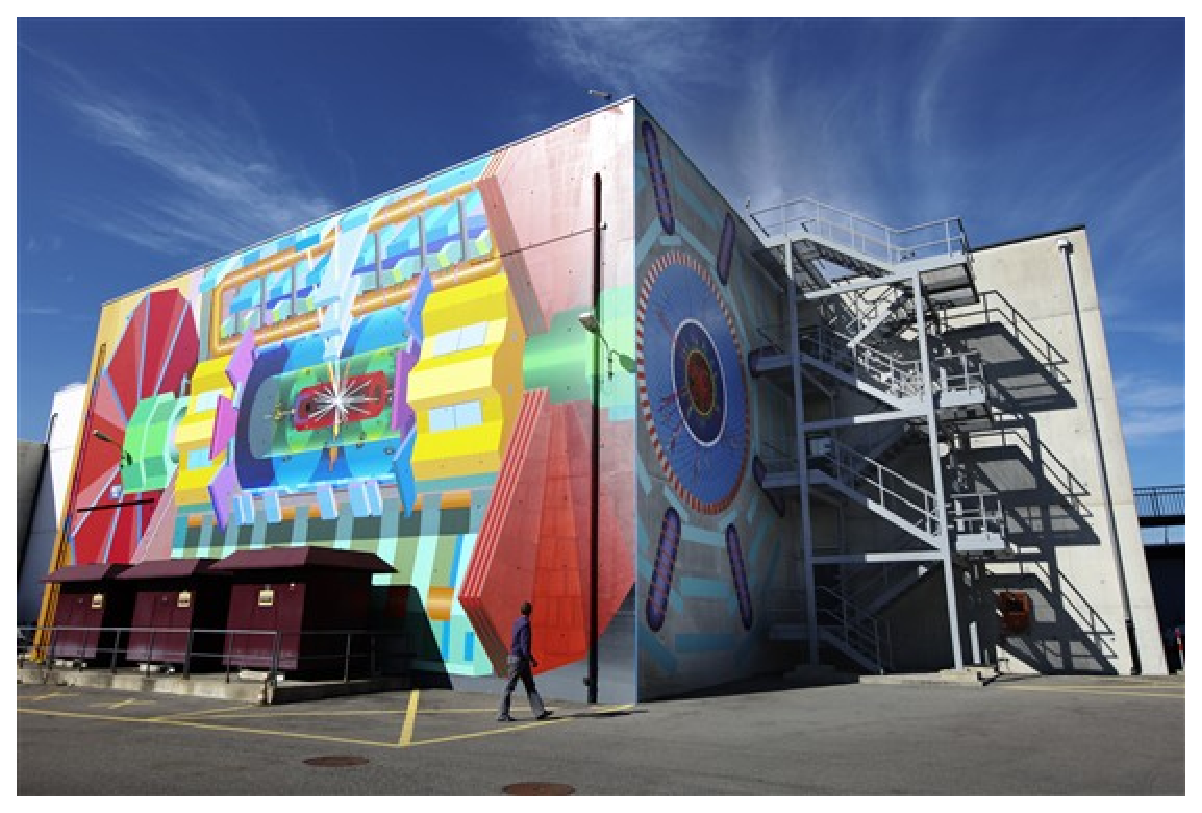
\includegraphics[width=0.47\textwidth]{detector/figures/mural}}
	\subfigure[]{\label{fig:lhcdraw}
  	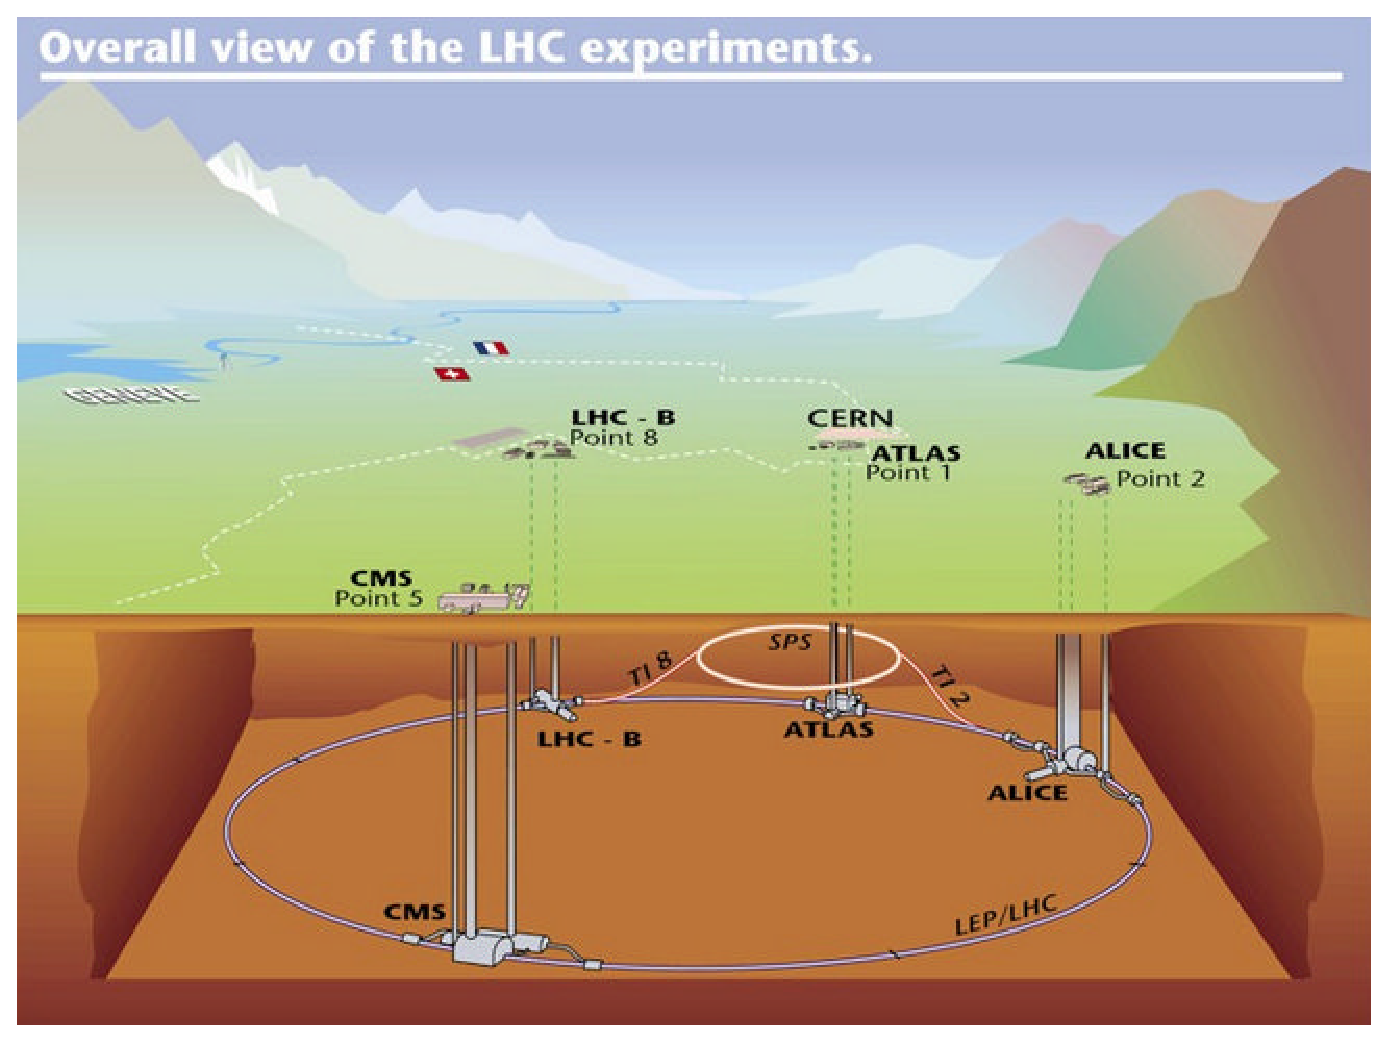
\includegraphics[width=0.42\textwidth]{detector/figures/lhc_diagram}}
	\caption[bla]{Left: View of Point 1, just above the ATLAS cavern, with a mural painting 
        of the detector, reproduced at a scale of about 1:3
        by artist Josef Kristofoletti\footnotemark.
        Right: A drawing of the LHC complex.\label{fig:nicepics}}
\end{center}\end{figure}

The collider accelerates protons up to 4~\tev, but is designed to reach 7~\tev\ per beam
when it will be operated at his full potential. This energy is achieved
through various steps, shown in Figure~\ref{fig:lhcring}.
To start with, protons are extracted from Hydrogen gas and injected in the first machine, the linear 
accelerator LINAC2 that starts the acceleration chain. When protons reach
an energy of 50~\mev\ they are injected into the Proton Synchrotron Booster
(PSB) and accelerated up to the energy of 1.4~\gev. The second circular
accelerator, the Proton Synchrotron (PS) brings the energy of the protons
to 25~\gev\ previous to injecting them into the last machine before the LHC,
the Super Proton Synchrotron (SPS). Protons of 450~\gev\ finally enter the
LHC where they are boosted to energies of up to 4~\tev.
The four main LHC experiments are shown on the collider ring.

\begin{figure}[tb]\begin{center}
	\subfigure{
  	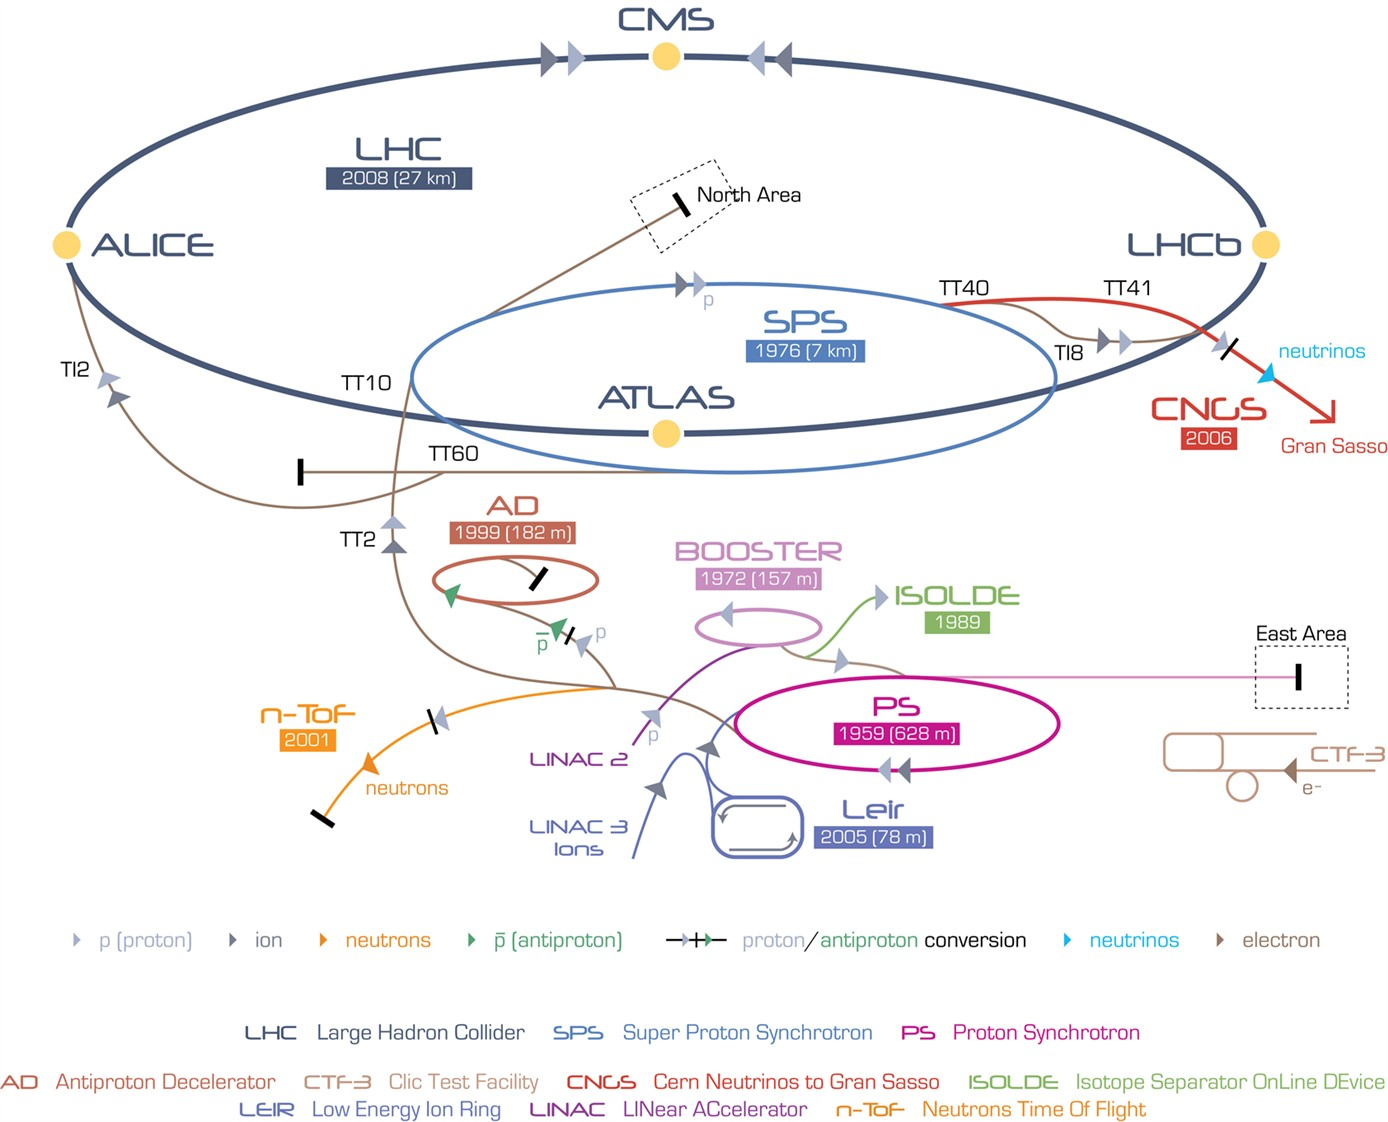
\includegraphics[width=0.8\textwidth]{detector/figures/ring.eps}}
	\caption{A schematic showing the accelerator complex at CERN.\label{fig:lhcring}}
\end{center}\end{figure}


\footnotetext{More info at: \url{http://www.atlas.ch/mural/}.}

The LHC is composed of eight arcs 2.7~km long, each of which contains 154 dipole 
magnets, whose function is to  bend the beams along the circular trajectory, and
49 quadrupole magnets, that focus the beam. These superconducting magnets operate
at a temperature of 1.9~K, maintained by means of liquid Helium vessels.
Eight insertions are placed inbetween the arches. Each insertion has a specific
role that characterizes its design and can be injection, beam dumping, beam cleaning,
or ``physics'', i.e. make the beams collide within an experiment.

First proton beams were circulated on 10th September 2008 and right on the verge of
getting the first collisions at a \cme $\rts=900\gev$ nine days later, an electrical
connection joining superconducting wires of a dipole and a quadrupole
failed. This caused the release of liquid Helium in the insulating vacuum,
resulting in an explosion that severely damaged the machine.
After more than one year devoted to repair the damage and consolidate the security,
on 30th November 2009 the LHC became the world's highest energy particle 
accelerator\footnote{\url{http://press.web.cern.ch/press/PressReleases/Releases2009/PR18.09E.html}}:
\begin{quotation}\small
Geneva, 30 November 2009. CERN's Large Hadron Collider has today become the world’s highest energy particle accelerator, having accelerated its twin beams of protons to an energy of 1.18 TeV in the early hours of the morning. This exceeds the previous world record of 0.98 TeV, which had been held by the US Fermi National Accelerator Laboratory’s Tevatron collider since 2001. It marks another important milestone on the road to first physics at the LHC in 2010.
\end{quotation}


One of the main characteristics for an accelerator is the luminosity, the 
instantaneous luminosity $\mathcal L$ being defined as 
\begin{equation}\label{eq:lumiN}
\mathcal{L}\times\sigma=\dfrac{dN}{dt}=f\times n\dfrac{N_1\times N_2}{A}\times\sigma.
\end{equation} 
Here $dN/dt $ is the event rate of a certain process and $\sigma$ is its cross 
section. This rate is directly proportional to the the frequency $f$, the number 
of bunches $n$ and the number of particles in the two bunches $N_1, N_2$, and
inversely proportional to the beam cross-section $A$.
The instantaneous luminosity is measured by dedicated subdetectors that are
described in Section~\ref{sec:forward}.

Integrating over the accelerator active time (a ``fill'', when stable beams are kept
colliding) gives the \textit{integrated luminosity}, relating the total number 
of produced events $N_{tot}$ to the cross-section:
\begin{equation}\label{eq:intLumi}
\int \mathcal L dt  = \dfrac{N_{tot}}{\sigma}.
\end{equation}




%http://accelconf.web.cern.ch/accelconf/IPAC2013/papers/moyab101.pdf
%http://cerncourier.com/cws/article/cern/54381

\begin{table}\centering
	\begin{tabular}{lllll}\toprule
        Parameter                       & designed      &       2010 &  2011     &   2012\\ \midrule
        Beam energy (\tev/c)            & 7             & 3.5        & 3.5       & 4    \\
        Beta function $\beta*$ (m)      & 0.55          & 2.0/3.5    & 1.5/1.0   & 0.6  \\
        Max. No. bunches/beam           & 2808          & 368        & 1380      &1380  \\
        Max. No. protons/bunch          & 1.15$\times10^{11}$ & 1.2$\times10^{11}$ & 1.45$\times10^{11}$ & 1.7$\times10^{11}$ \\
        Bunch spacing (ns)              & 25            & 150       & 75/50        & 50 \\
        Peak luminosity (\cmm2\sm1)     & 1$\times10^{34}$& 2.1$\times10^{32}$& 3.7$\times10^{33}$& 7.7$\times10^{33}$\\
        Emittance $\varepsilon_{n}$ ($\mu$rad)&3.75     &   2.0      & 2.4      & 2.5   \\
        Max. $<\mu>$                    & 19            & 4             & 17         & 37       \\
	\bottomrule\end{tabular}\caption{Overview of some parameters for the LHC performance comparing the design values with their time
        evolution during the first long run operation in 2010-2013~\cite{Lamont}.}\label{tab:lhcpar}
\end{table}

\begin{figure}[tb]\begin{center}
	\subfigure[]{\label{fig:intlumi}
  	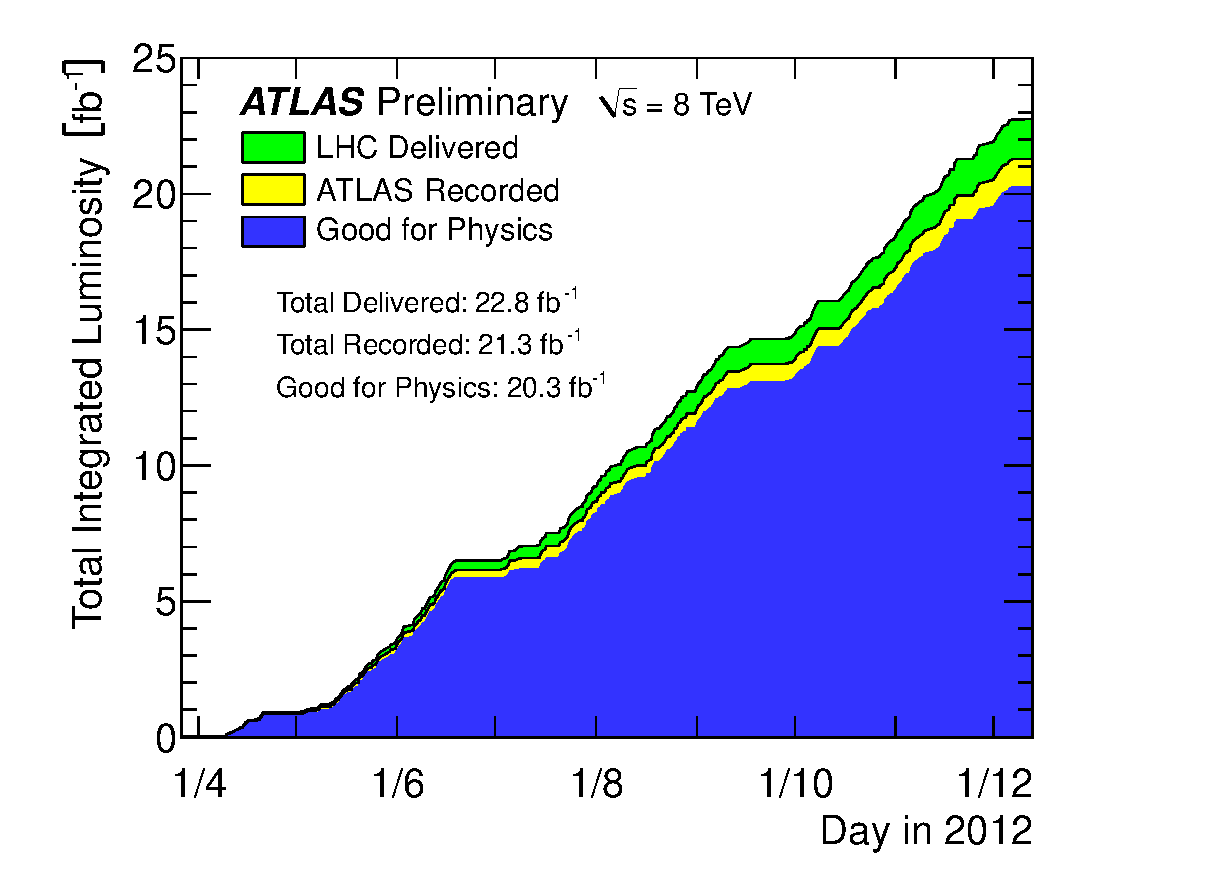
\includegraphics[width=0.48\textwidth]{detector/figures/intlumivstime2012DQ}}
	\subfigure[]{\label{fig:mu}
  	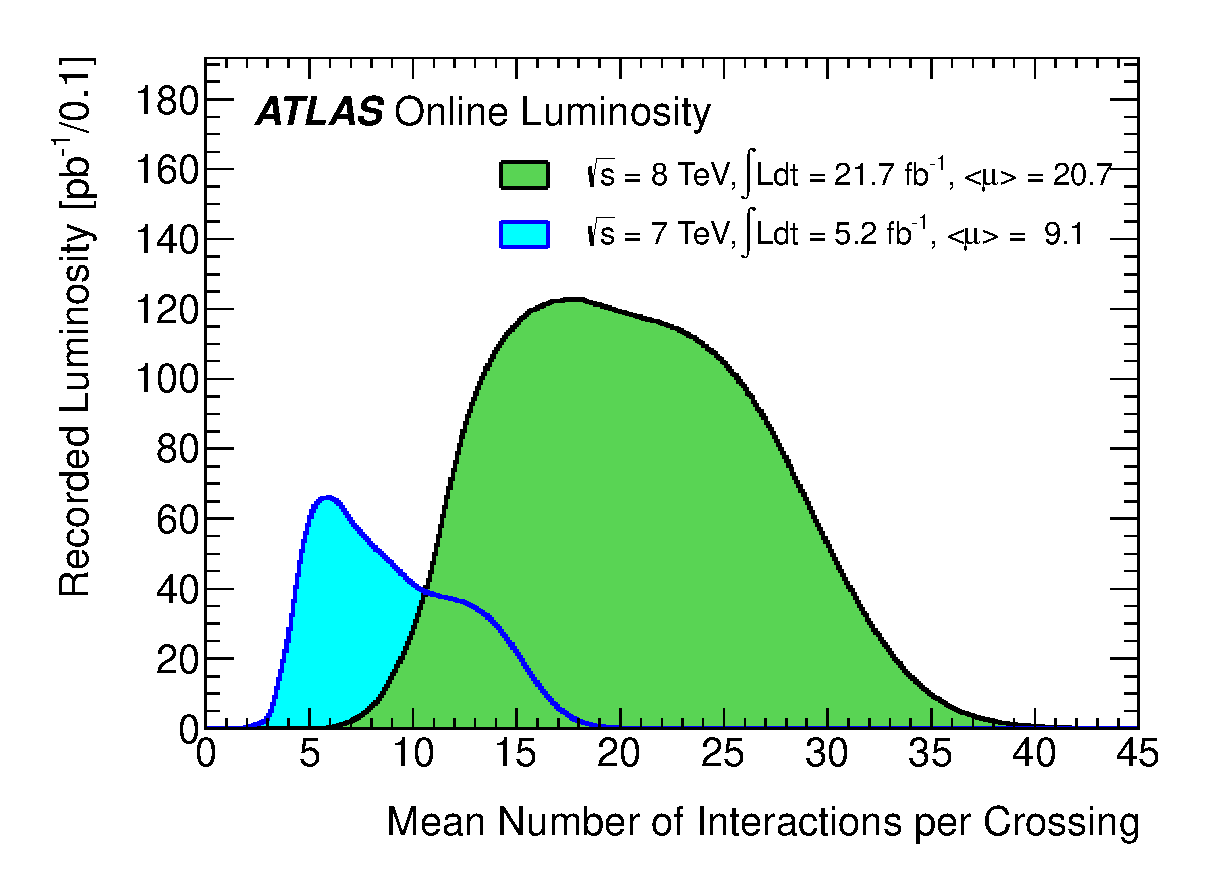
\includegraphics[width=0.48\textwidth]{detector/figures/mu_2011_2012-dec}}
	\caption{(a) Total integrated luminosity versus time delivered by the LHC to ATLAS (in green), recorded by the experiment 
        (in yellow) and selected as ``good data'' for analysis (in blue) for p-p collisions at \rts=8~\tev.
        (b) Mean number of interactions per beam crossing during 2011 and 2012 LHC runs, where 
        $\mu = \mathcal L\times \sigma_{\rm inelastic}/f$ depends on the instantaneous luminosity $\mathcal L$, the p-p inelastic
        cross section $\sigma_{\rm inelastic}$ and the revolution frequency $f$.~\cite{lumi}}
%Number of Interactions per CrossingMore details on this can be found in arXiv:1101.2185. 
\end{center}\end{figure}

In 2010 ATLAS collected about 45~\ipb of p-p collision data at \rts=7~\tev, and in
2011 reached about 5~\ifb of the same data.
In 2012, with  \rts=8~\tev\ collisions, LHC reached a peak luminosity of 7.7$\times10^{33}$~\cmm2\sm1\ which is
more than half the design luminosity, as shown in Table~\ref{tab:lhcpar} together
with other parameters relevant for the accelerator performance. 
Over 2012, the last
year of data taking before the long shutdown\footnote{LHC terminated the p-p program
at the end of 2012, operated proton-heavy ion collisions for two months at the beginning
of 2013 and then stopped for what is called the first long shutdown. During this two-years
time the accelerator and the experiments as well will undergo substantial maintenance and 
upgrade works, in order to be re-operated in 2015 with higher performance at a higher
\cme for particle collisions.},
ATLAS collected about 20~\ifb\ of p-p collision data at \rts=8~\tev.
Figure~\ref{fig:intlumi} shows the delivered luminosity from the start of stable beams until beam dump and the luminosity recorded by
ATLAS during stable beam conditions, the difference with respect to the delivered luminosity being due to Data AQuisition (DAQ)
inefficiencies. Of the recorded luminosity, only a part is usable for analysis, and is what is called ``good data'', i.e. 
the data that satisfy Data Quality (DQ) requirements assessed after reprocessing (see Section~\ref{sec:daq}).

In order to increase the luminosity LHC operates with a high number of protons per bunch as well as a high
 number of bunches per beam and reduces the inter-bunch latency time.
This overall defines a set of challenges that physics analysis will face associated to the high luminosity.
Even at the detector design stage, the high frequency of collision environment foreseen influenced
the choice of radiation resistance material for the experiment sub-systems. Concerning directly the physics
%instead we can list the main problematics as being \textit{underlying events} and \textit{pile-up}
instead, the main problematic is \textit{pile-up}.

Pile-up events are distinguished between \textit{in-time} and \textit{out-of-time} pile-up. The first ones come 
from the multiple inelastic scatterings of protons in the same bunch, as if we consider a cross-section of 80~mb
at the nominal luminosity of $10^{34}$~\cmm2\sm1 the number of events per second will be something like
a billion. This translate, at a collision frequency of one crossing every 25~ns, to about 20 interactions per
crossing that will be detected simultaneously. A useful observable to estimate in-time pile-up is
the number of reconstructed primary vertices (see Section~\ref{sec:primaryvertex}) $N_{\rm PV}$.
In addition, on the other hand, the inter-bunch time interval is so short
that the electronics reading the detector might not keep up with the frequency of collisions, leading to the
cumulation of events that happened in different beam crossings. This is the effect we refer to as 
out-of-time pile-up, and a good estimator for it is the average number of p-p interactions
per bunch crossing at the time of the event, $<\mu>$, which recalling Equation~\ref{eq:lumiN} is defined as:
\begin{equation}\label{eq:mu}
<\mu> = \dfrac{LA}{nf},
\end{equation}
with $L$ being the average instantaneous luminosity over a time period $\Delta t\gg 600$~ns.
The maximum values reached by the variable $<\mu>$ during the three years of data taking
are reported in Table~\ref{tab:lhcpar}.

Finally, ATLAS makes use of a three-level trigger system (described in Section~\ref{sec:trigger}) to identify
and record only the events of interest, while the pile-up issues are dealt with at the analysis 
reconstruction level.



\section{The ATLAS detector}\label{sec:atlas}

ATLAS (A Toroidal LHC ApparatuS)~\cite{Aad:2008zzm} is a general purpose experiment
aimed at exploring a vast range of physics scenarios and designed to measure the particles
produced in p-p collisions at the LHC at unprecedented energies and instantaneous luminosities. 
It is the biggest detector of its kind ever built (it's 46~m long and 25~m high) is characterized by
a full coverage of the space around the p-p interaction point and complete
containment of the particles produced in the collision. Different subsystems are
layered concentrically one after the other, each of them pursuing a specific task. 
Right around the interaction point
(IP) where the LHC makes protons collide there is the Vertex Detector, reconstructing
charged particles trajectories that are bent by the first solenoid magnet surrounding
the Vertex Detector. Particles going through it then encounter the two calorimeter systems,
the Electromagnetic and the Hadronic one. Muons are the only particles that will pass
the calorimeters material (beyond neutrinos) and a dedicated Muon Spectrometer is the last
piece of detector, embedded in a huge toroidal magnet. The detector complex is presented
as a schematic in Figure~\ref{fig:atlas}, and a drawing of particle detection in the various
subdetector systems is shown in Figure~\ref{fig:detection}. 

\begin{figure}[htb]\begin{center}
	\subfigure{
  	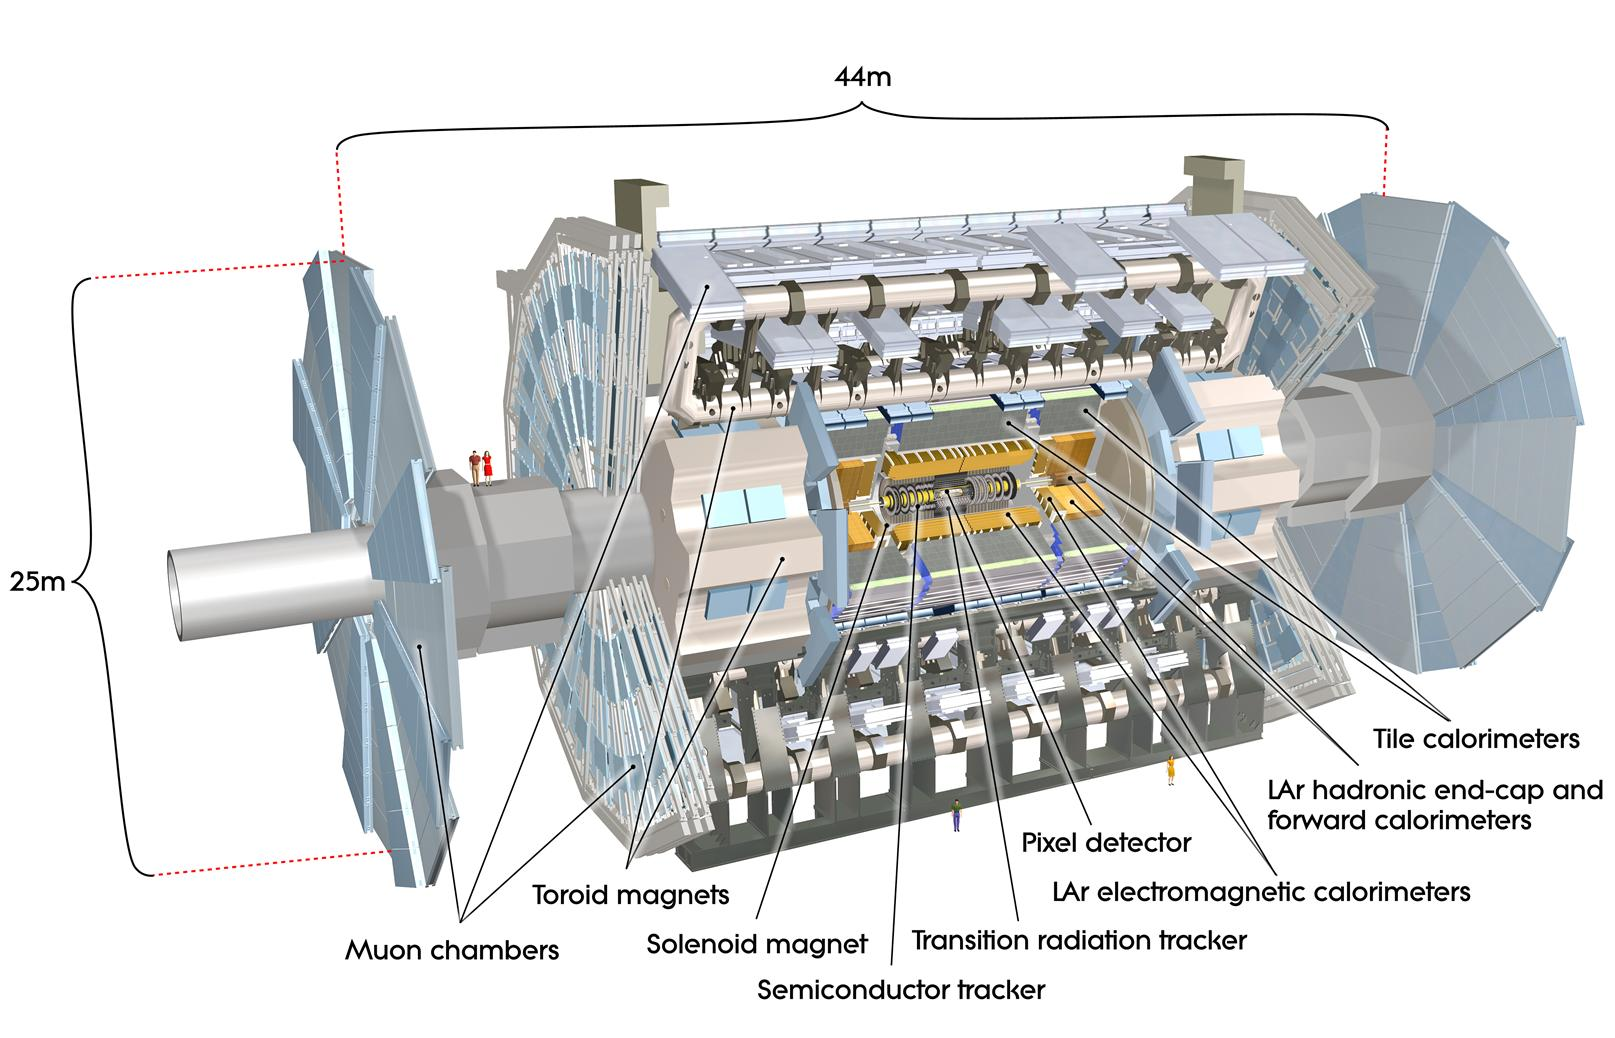
\includegraphics[width=0.9\textwidth]{detector/figures/atlas}}
	\caption{Schematic drawing of the ATLAS experiment. The detector subsystem are indicated as well as the total dimensions.\label{fig:atlas}}
\end{center}\end{figure}

\begin{figure}[htb]\begin{center}
	\subfigure{
  	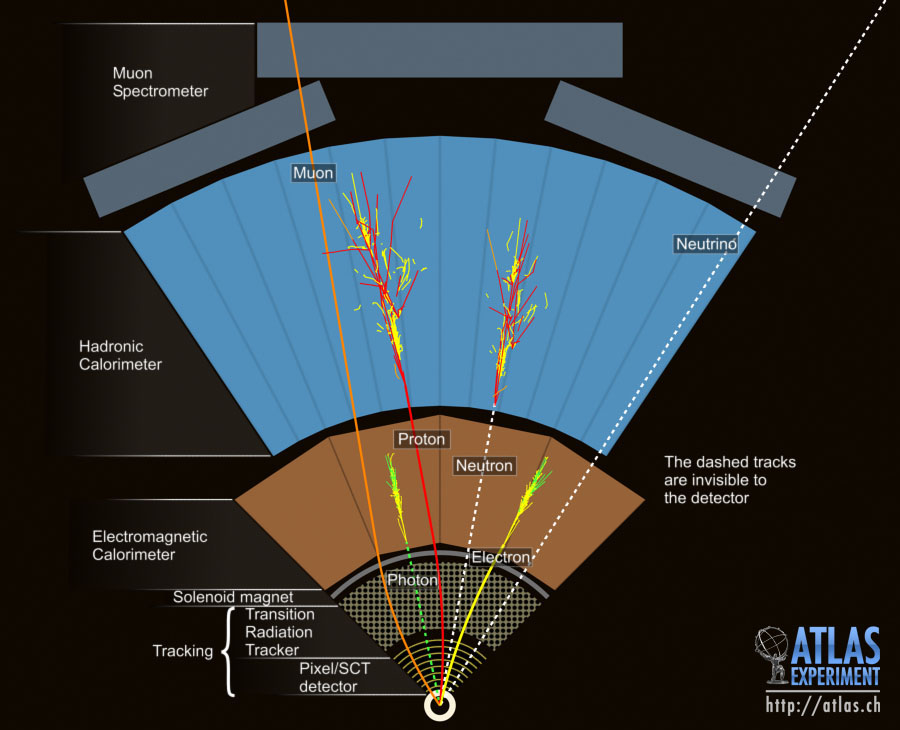
\includegraphics[width=0.75\textwidth]{detector/figures/detection}}
	\caption{Drawing of the detection of particles going from the interaction point through the whole detector.\label{fig:detection}}
\end{center}\end{figure}


\subsection{Coordinate system}

Protons from the two circulating beams are made to collide in the center of the ATLAS detector, in the region
that takes the name of Interaction Point (IP). The IP is taken as the origin of a three dimensional XYZ right-handed
coordinate system. The Z axis is tangent to the trajectory of the beams while the XY plane is perpendicular to
it and defines a symmetry plane for the detector, dividing it into the $A$ and $C$ sectors, respectively in the
positive and negative Z semi-axes. Figure~\ref{fig:coord} shows a schematic of the coordinate system.

\begin{figure}[tb]\begin{center}
	\subfigure[]{\label{fig:coord}
  	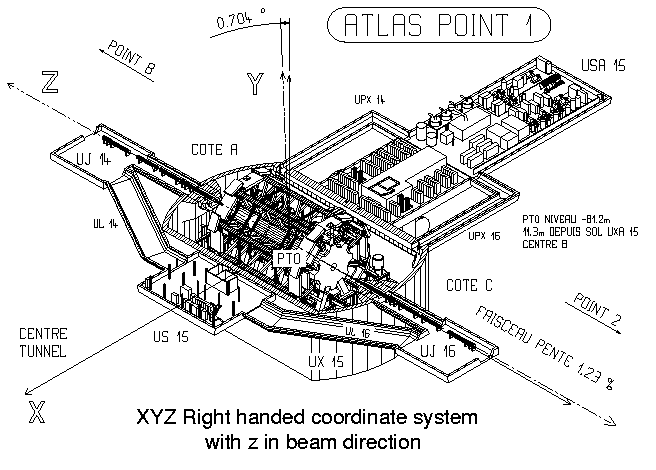
\includegraphics[width=0.6\textwidth]{detector/figures/coord}}\hskip3ex
        \subfigure[]{\label{fig:spherical}
  	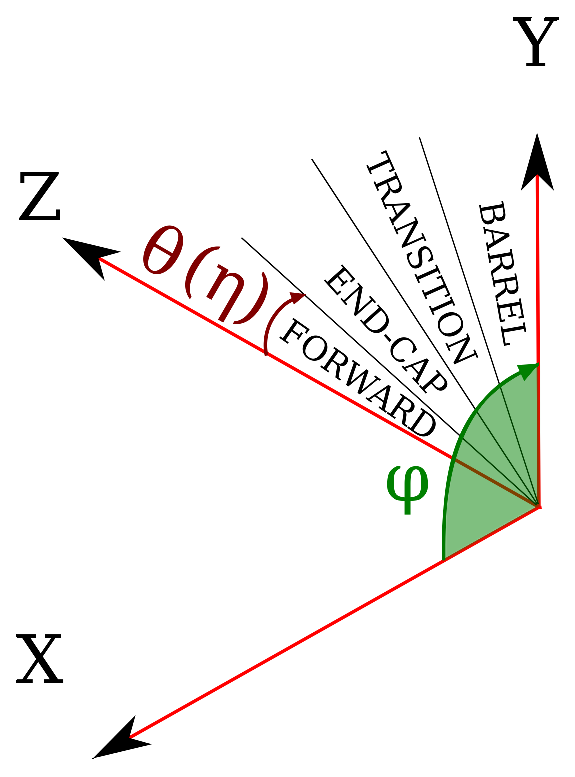
\includegraphics[width=0.3\textwidth]{detector/figures/spherical}}
	\caption{(a) Drawing of the ATLAS experiment with the cartesian coordinate system. The positive X axis points towards the center of the LHC
        ring. The positive Z axis points todards the anti-clockwise circulating direction of beam 2. (b) Simple schematic showing the spherical coordinates and the
        region definition in terms of the absolute value of the pseudorapidity $\eta$. These regions are symmetrical with respect to the transverse
        XY plane.}
\end{center}\end{figure}

In terms of polar coordinates, the Z axis is again along the beam axis and in the transverse plane 
the $R$ and $\phi$ coordinates are defined with $\phi$ ranging between 
$-\pi$ and $+\pi$ with respect to the X axis. In terms or spherical coordinates (see Figure~\ref{fig:spherical}),
the radial vector $R$ originates from the IP,  the azimuth $\phi$
is the same as the polar angle $\phi$, 
and the polar angle $\theta$ is measured with respect to the Z axis and
ranges between 0 and $\pi$. 

Since the interaction initial energy is unknown, being dependent on the parton distribution functions for the proton
energy, it is useful to define the transverse component of variables of 
interest\footnote{These quantities transverse initial value will be, indeed, zero, as the protons are accelerated along the Z axis.}  
like the energy and the momentum, being taken as the projection on the XY plane:

\begin{equation}\label{eq:transv}
\et = E\sin\theta, \qquad \pt = p\sin\theta.
	\end{equation}

Another common variable used at hadron colliders to describe the polar distribution and preferred to the simple
polar angle $\theta$ is the pseudorapidity $\eta$:
\begin{equation}\label{eq:pseudorapidity}
        \eta \equiv -\ln\bigg(\tan\frac{\theta}{2}\bigg);
	\end{equation}
which, for relativistic regimes, is equal to the rapidity $y$:
\begin{equation}\label{eq:rapidity}
y \equiv \frac{1}{2} \ln \bigg(\frac{E+p_{Z}}{E-p_{Z}}\bigg);
	\end{equation}
and $\Delta y$ and $\Delta \eta$ are Lorentz invariant. The pseudorapidity is preferred
to the rapidity as it does not require knowing the particle mass but only its polar position.
The distance between two particles is often referred to in terms of $\Delta R$:
\begin{equation}\label{eq:deltar}
\Delta R = \sqrt{(\Delta\eta)^{2} + (\Delta\phi)^{2}}.
	\end{equation}


%since particles produced in collisions are not uniformely distributed in $\theta$. 
Figure~\ref{fig:spherical} shows how different pseudorapidity regions are named. Particles
along the Z axis have a pseudorapidity $|\eta|=\infty$, particles along the Y axis have
a pseudorapidity $|\eta|=0$. ATLAS has an excellent hermeticity and is able to cover 
pseudorapity regions up to $|\eta|=4.9$. Typically, physics analysis consider objects in
the pseudorapity region  $|\eta|<2.5$. For a quick visualization of the correspondence
in terms of polar angle distribution, some pseudorapidity values are reported in Table~\ref{tab:etatheta}.
%AAAAAAAAAAAAAAAAA add barrel forward blabla exact def


\begin{table}[htb]\centering\begin{tabular}{cccccccccc}\toprule
$\theta$ & 0$^{\circ}$ & 5$^{\circ}$ & 10$^{\circ}$ & 20$^{\circ}$ & 30$^{\circ}$ & 45$^{\circ}$ & 60$^{\circ}$ & 80$^{\circ}$ & 90$^{\circ}$ \\
$\eta$ & $\infty$ & 3.13 & 2.44 & 1.74 & 1.31 & 0.88 & 0.55 & 0.175 & 0\\\bottomrule \end{tabular}
\caption{Pseudorapidity vs polar angle values.}\label{tab:etatheta}\end{table}

\subsection{Magnets}\label{sec:magnets}

ATLAS is provided with four superconducting magnets that allow the measurement of
charged particles momenta by curving their trajectory. 

A central solenoid, 5.3~m long and 2.4~m in diameter, sits 
around the inner detector and produces a 2~T magnetic field along the direction
parallel to the beam axis. It is only 45~mm thick (equivalent to 0.66 radiation lenghts $X_0$)
and is cooled with liquid Helium, sharing the cryostat with the electromagnetic calorimeter.

Paired to the muon spectrometer, the superconducting air-core toroid magnet (Figure~\ref{magnets}) 
has an open structure with eight superconducting toroidal coils in the barrel part (each 25.3~m long, located
at the outer diameter of 20.1~m) and
two end-cap systems made of eight coils. The field strength varies strongly with $\phi$:
in the barrel region ($|\eta|<1.4$) is 1.5-5.5 Tesla$\cdot$m; in the end-caps ($1.6<|\eta|<2.7$) 1-7.5 is Tesla$\cdot$m. 
Such configuration of the magnets gives a field orthogonal to the muons trajectory.

\begin{figure}[hbt]\begin{center}
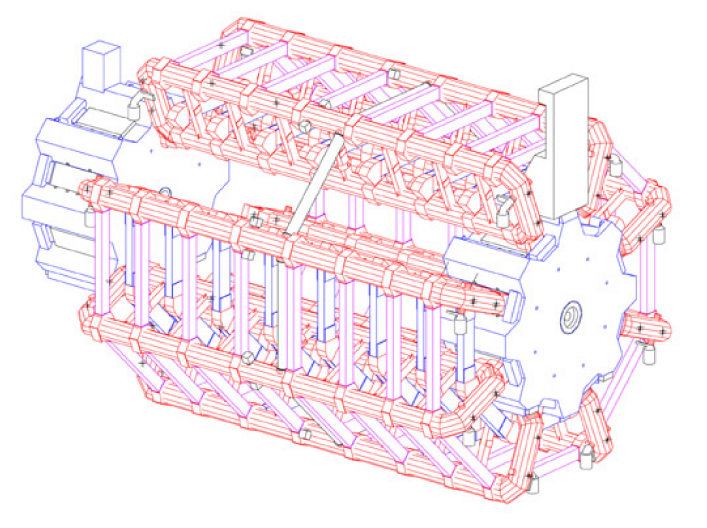
\includegraphics[width=.8\textwidth]{detector/figures/magnets}\caption{Toroidal magnet system.}\label{magnets}
\end{center}\end{figure}



\subsection{Inner detector}\label{sec:innerdet}

The Inner Detector (ID) is the subsystem closest to the IP and tracking charged particles arising from collisions allows for 
the measurement of their momentum and vertex reconstruction with excellent resolution. At the design choices level, radiation resistance had to
be taken into account, as well as reducing the amount of material to be placed in front of the calorimeters to avoid spoiling the energy measurement.
This quantity varies between 0.5 and 2.5~$X_0$ depending on the pseudorapidity region, most of it coming from supporting equipment. This material
is responsible for photon conversions and electron bremsstrahlung.

The ID is surrounded by the central solenoid magnet (Section~\ref{sec:magnets}) and is composed by three subsystems, 
from the closest to the furthest from the IP: the pixel detector, the SemiConductor Tracker (SCT) and
the Transition Radiation Tracker (TRT).
%silicon strip detector and a straw detector (Figures~\ref{fig:innerdet1} and~\ref{fig:innerdet2}).

\begin{figure}[tb]\begin{center}
	\subfigure[]{\label{fig:innerdet1}
  	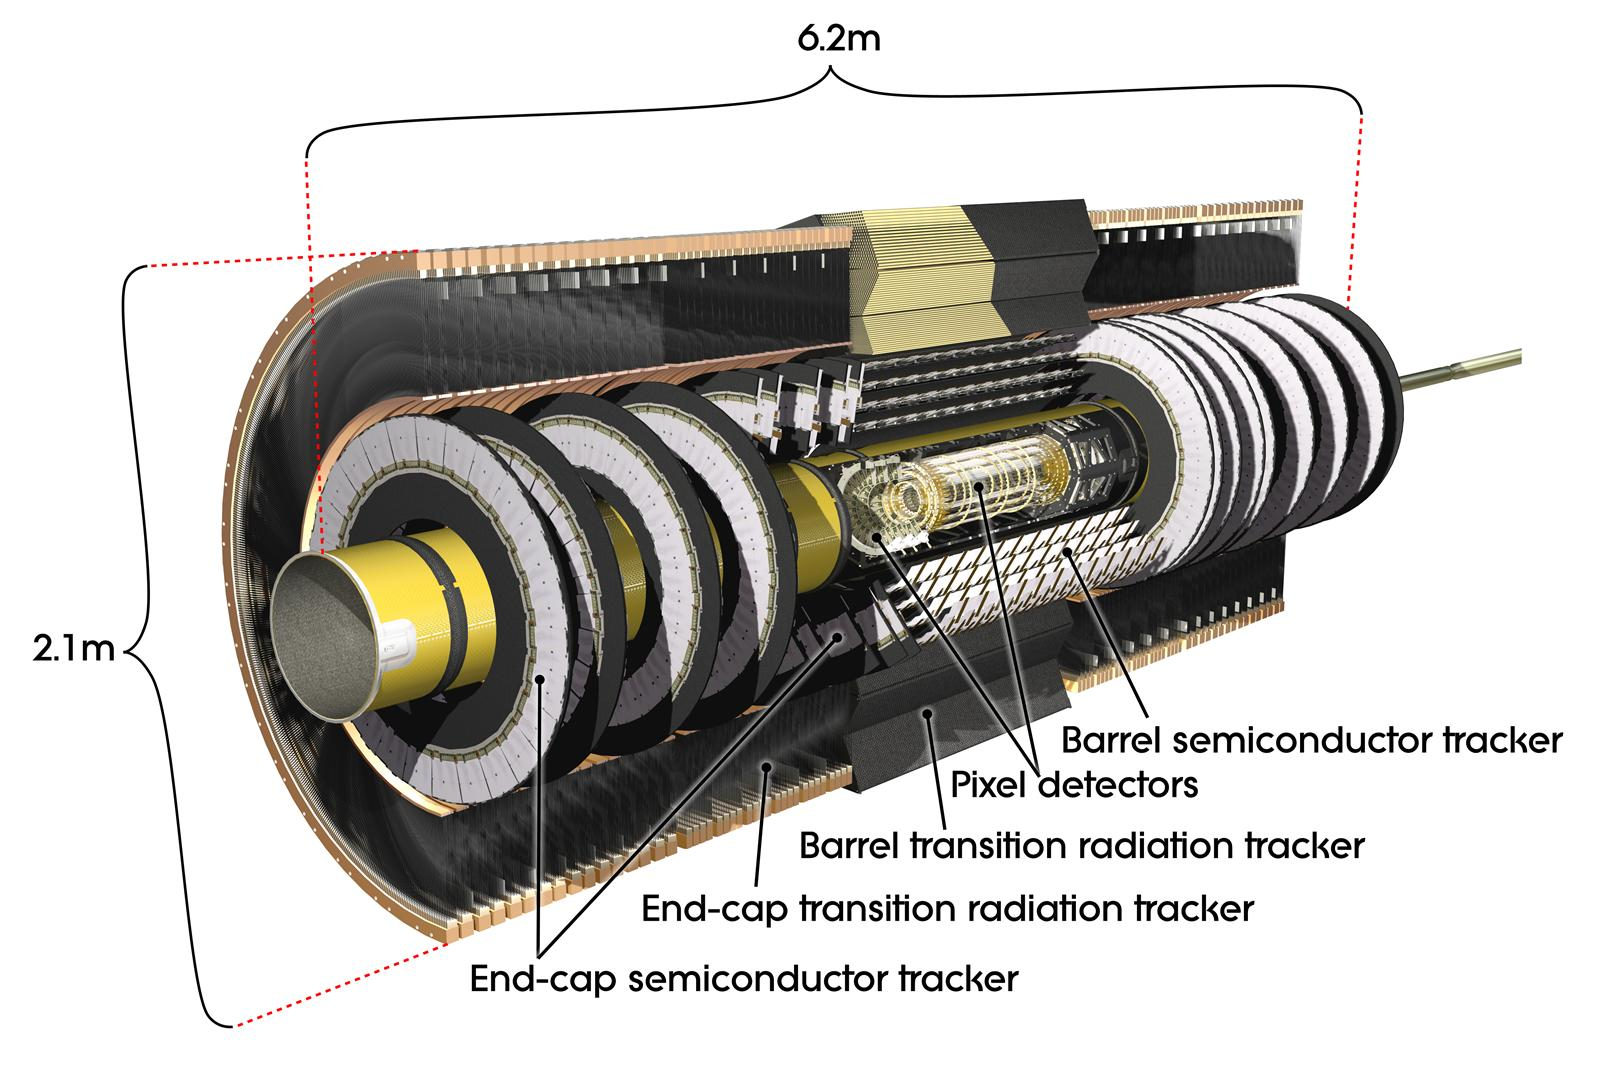
\includegraphics[width=0.6\textwidth]{detector/figures/innerdet}}
	\subfigure[]{\label{fig:innerdet2}
  	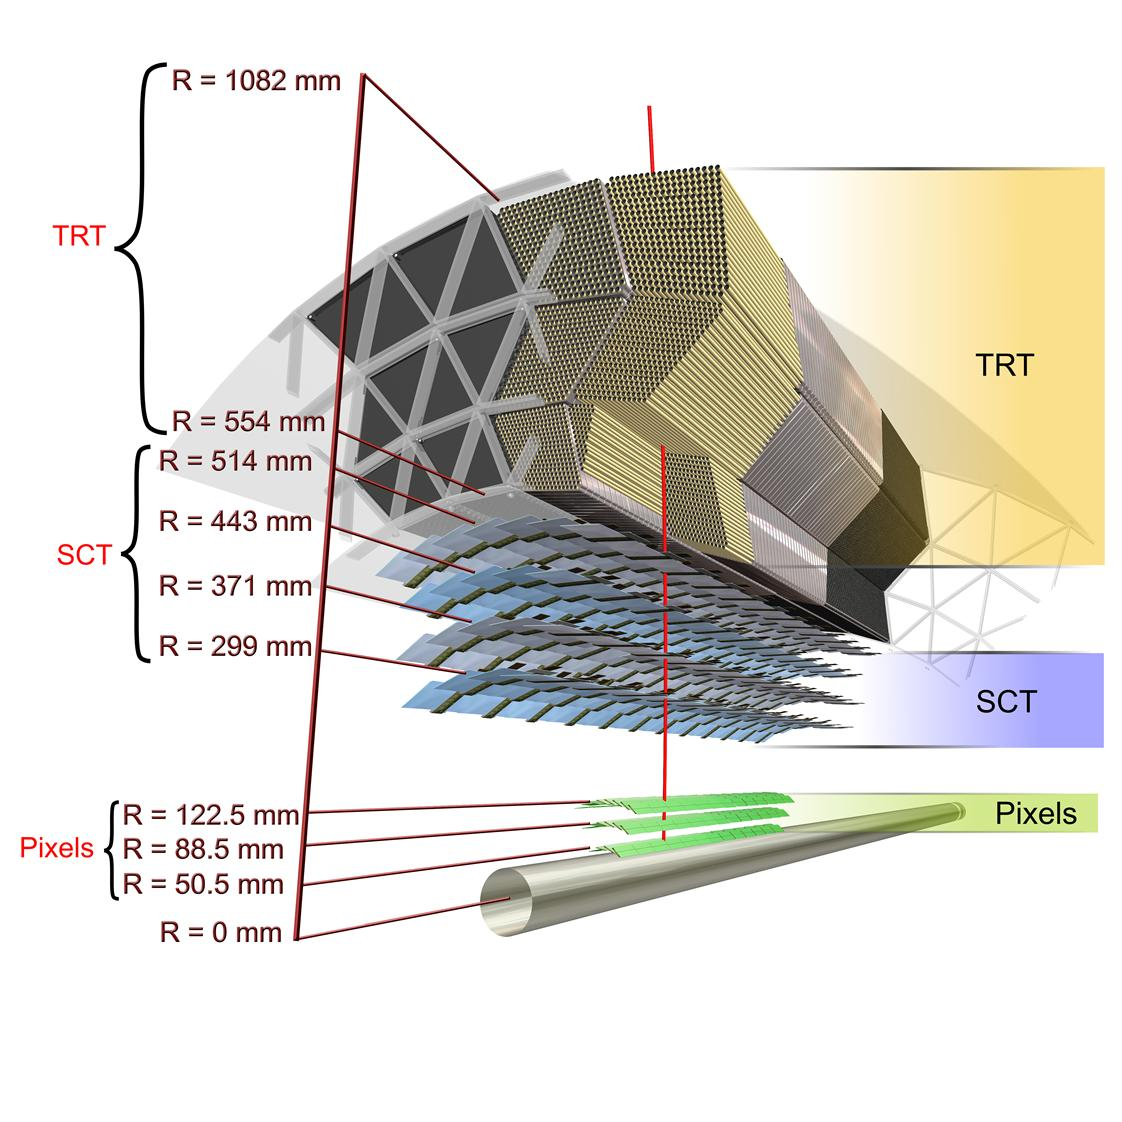
\includegraphics[width=0.37\textwidth]{detector/figures/innerSection}}
	\caption{(a) Schematic of the ID system. (b) Detailed schematic of the barrel section of the ID showing the
        three subsystems and reporting the distance to the center of the beam pipe.}
\end{center}\end{figure}


\subsubsection{Pixel detector}

The first subsystem covers the region $|\eta|<2.5$ and  is composed by three cylindrical layers in the barrel region, each of them distant from the beam by
50.5~mm, 88.5~mm and 122.5~mm respectively, and by three concentric discs in the end-cap region, each of them distant from the beam by
49.5~mm, 58.0~mm and 65.0~mm respectively.
Each silicon pixel has a size of 50$\times$400~$\mu$m$^{2}$ and is 250~$\mu$m thick, 
with in total $\sim$80.4 million readout channels to achieve a very fine granularity.
The precision is of 10~$\mu$m in $R\phi$ and 115~$\mu$m in Z and $R$ in the barrel and end-cap
region respectively.

The very first layer is called $B-$layer as, thanks to its position really close to the IP,
allows for the reconstruction of secondary vertices associated with the production of
 short lived particles such as $B-$hadrons. This information is very useful to identify
jets originating from the fragmentation of $b$ quarks.

\subsubsection{Semiconductor tracker}

After the three layers of pixel detectors, come four layers of  silicon strip detectors. The SemiConductor
Tracker (SCT) also covers the region $|\eta|<2.5$ with a barrel and end-cap design similar to the 
pixel detector one, being composed by eight silicon strips (two per layer) 128~mm long and 80~$\mu$m large.
It makes use of $\sim$6.3 millions readout channels and the resolution achieved is of 17~$\mu$m 
in $R\phi$  and 580~$\mu$m in Z ($R$) in the barrel (end-cap) region.

By allowing for four redundant position measurements\footnote{One of the coupled layers is rotated of $40$mrad with respect
to the other, which is parallel to the axis, giving a small stereo angle for a redundancy in the $\phi$ coordinate measurement.}, 
the SCT contributes mainly to the momentum reconstruction.

%Silicon has a band gap of just 3.6 eV, that is the minimum energy to create an electron/hole pair. Thus a minimum ionising particle creates around 80 electron/hole pairs per $\mu$m through primary and secondary ionisation.

\subsubsection{Transition Radiation Tracker}

In order to reduce the amount of material in front of the calorimeters, and to reduce the construction costs as well,
in the third subsystem the semiconductor technology has been substituted with straw detectors.
The Transition Radiation Tracker (TRT) consists of thin proportional chambers made of straw polyimide drift tubes, 4~mm in diameter.
The drift tubes are filled with a gas mixture composed of: 70\% Xenon, 27\% Carbon Dyoxide, 3\% Oxygen. The anode 
collecting the electrons from the ionized gas at the passage of the charged particle is made of
tungsten covered in gold.

In the barrel region the tubes are 144~cm long and placed parallel to the beam axis, while in the 
end-cap region they are 37~cm long and positioned radially in wheels, with layers of radiator foils alternated 
to layers of straws. The resolution achieved is of 130~$\mu$m in $R\phi$ and Z$\phi$  in the two regions respectively.
The covered pseudorapidity region is of $|\eta|<2.0$ and the readout is composed by $\sim$351000 channels.

About 36 measurements per track are taken, and since each channel provides two independent thresholds per hit,
it is possible to discriminate between electrons and pions, since the former will more likely reach the
high threshold.

In the end, the combination of the three ID subsystems gives very precise $R\phi$ and Z measurements, as well as good track pattern recognition.
The resolution on the transverse momentum, measured with cosmic muon calibration runs~\cite{id_cosmic}, is:

\begin{equation}\label{eq:momentumres}
\frac{\sigma_{\pt}}{\pt}=P_1 \oplus P_2 \times \pt,
	\end{equation}
where $P_1=1.6\pm0.1\%$ and $P_2=(53\pm2)\times10^{-5}$~\GeV$^{-1}$. This means a 
resolution of~$\sim$1.6\% for tracks with $\pt\sim$1~\GeV\ and 
$\sim$50\% for tracks with $\pt\sim$1~\tev.


\subsection{Calorimeters}\label{sec:calo}

Particles leaving the ID and surviving the crossing of the central solenoid magnet
will face the calorimeter system, depicted in Figure~\ref{fig:calorimeters}.
The full system is characterized by a coverage
in pseudorapidity up to $|\eta|<5$ and an almost full coverage in $\phi$. With its 
22~$X_0$ and 24~$X_0$ radiation lengths of material in the barrel and end-cap regions respectively 
it is also able to stop most of the non-muon particles from the interaction.
Besides particles energy measurement, the calorimeters provide particle identification
information, discriminating electrons, photons and jets, and the determination
of the missing transverse energy.

Different technologies are used in the barrel, end-cap and forward regions for both the
electromagnetic and the hadronic calorimeters. All of them are sampling calorimeters,
with a dense medium acting as absorber to stop particles and start showers, and an
active material to detect the signal from ionization. For the electromagnetic calorimeters
and the forward hadronic calorimeter liquid argon is used as active medium, while the
barrel and extended-barrel hadronic calorimeter uses scintillating tiles.
The liquid argon is cooled at a temperature of about 88~K, with the use of two sets of cryostats:
the barrel electromagnetic calorimeter shares the cryostat with the central solenoid;
the end-cap and forward electromagnetic calorimeter and the hadronic end-cap calorimeter
share a cryostat in the foward region.

\begin{figure}[tb]\begin{center}
	\subfigure{
  	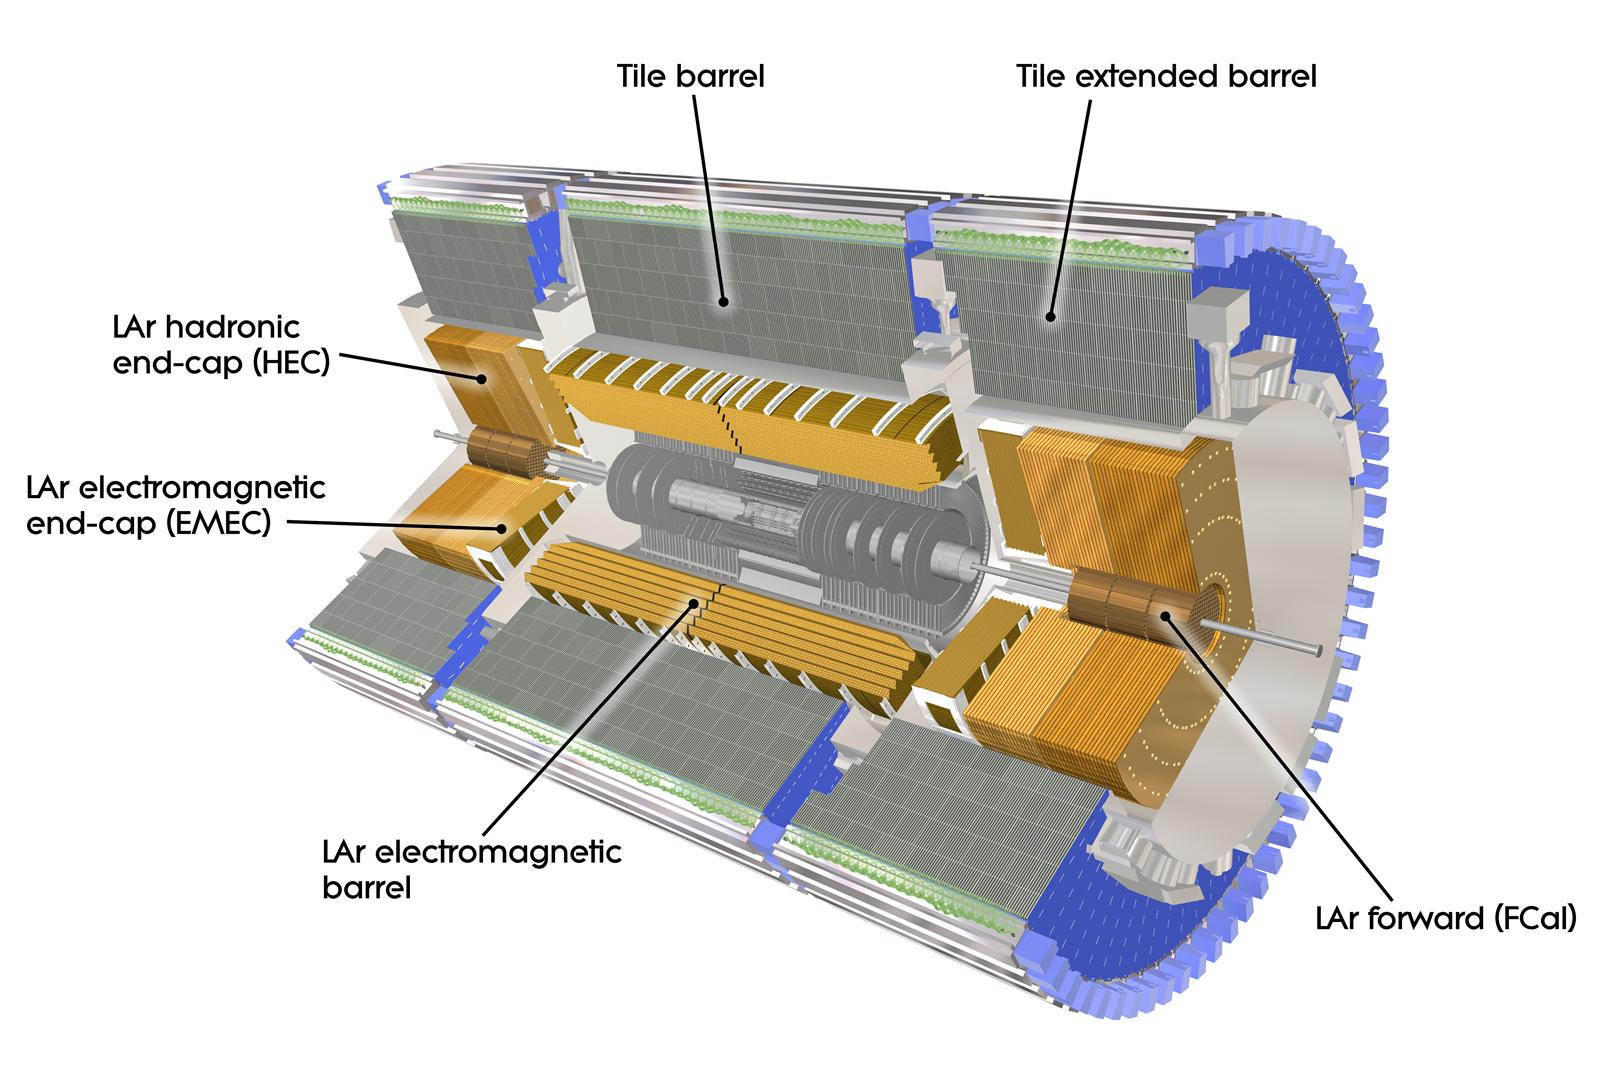
\includegraphics[width=0.8\textwidth]{detector/figures/caloBarrel}}
	\caption{Schematic of the calorimeter complex of the ATLAS detector.\label{fig:calorimeters}}
\end{center}\end{figure}

Particles interact both with the passive and active material, but only the energy released
in the active samples will be detected. 
%The balance, chosen at the design stage, between
%the two elements will determine how much the calorimenter compensate for the 
The processes involved in the shower formation are several and mainly electromagnetic.
Photons in matter can undergo the photoelectric effect, Compton scattering and $\gamma \to \epem$
pair formation. The general contribution of these processes depends both on the photon energy
and on the atomic number $Z$ of the material, and is shown in Figure~\ref{fig:photonsmatter}.
Electrons and positrons can ionize atoms and molecules, produce bremsstrahlung $\epm \to \epm + \gamma$
and emit Cerenkov radiation. Unless the calorimeter has been specifically designed for it,
 Cerenkov radiation does not contribute much, while ionization is the main process for energies
up to $\sim 100$~\mev, where bremsstrahlung starts to dominate.

In general, these cascade of events
continues until a certain threshold is reached, and the final number of particles
produced is proportional to the energy of the first particle originating the shower.

\begin{figure}[tb]\begin{center}
	\subfigure{
  	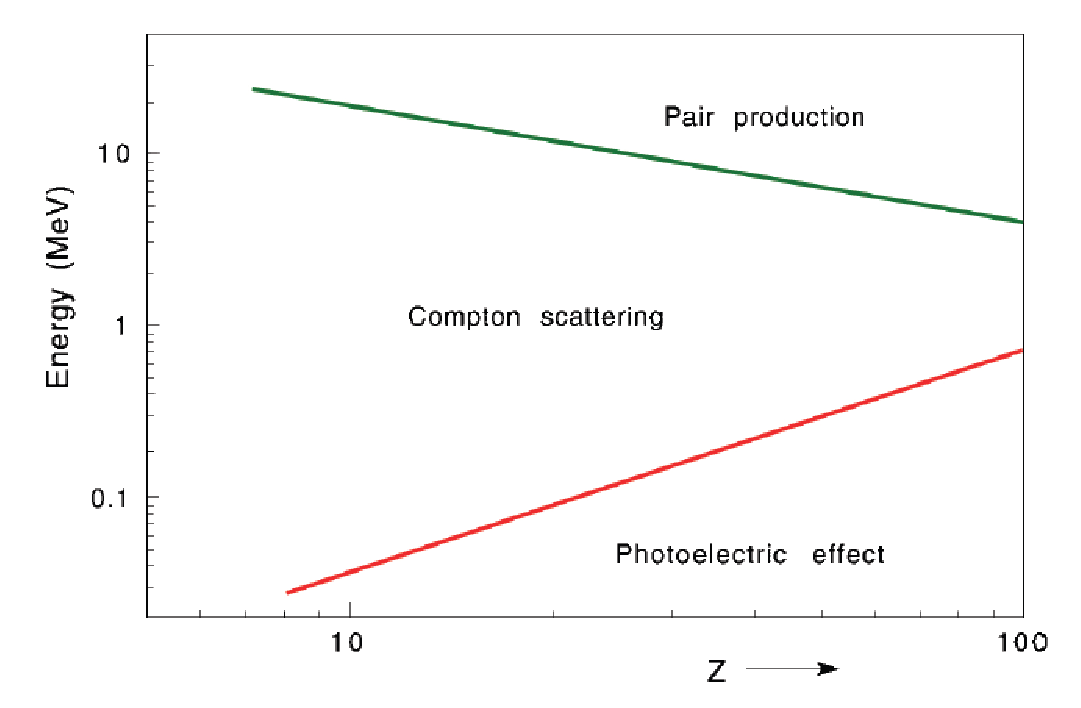
\includegraphics[width=0.6\textwidth]{detector/figures/photonsmatter}}
	\caption{Domains in term of photon energy and $Z$ number of the absorber material
        in which photoelectric effect, Compton scattering and pair production are the 
        favorite processes for energy loss~\cite{Wigmans}.\label{fig:photonsmatter}}
\end{center}\end{figure}

Also hadrons interact with matter, either ionizing it (if charged) or by nuclear interactions.
The problem of the latter process is that this energy release is often not directly detectable,
like in nuclear breakups and excitations, and is therefore called ``invisible energy''.
Secondary hadrons will be produced, forming the hadronic part of the shower, but sooner
or later something like $\pi^0\to \gamma\gamma$ will happen and the shower will
develop electromagnetically further on.

The average fraction of electromagnetic and hadronic shower components is a characteristic
of the sampling calorimeter and depends on the choice of the passive and active material
and on the design. Calorimeters are said to be {\it non-compensating} if, like the ATLAS
calorimeters, the detection of hadronic showers is less efficient than the one of 
electromagnetic showers. Calorimeters with a similar response for the two components
are called  {\it compensating}, while calorimeters more efficient when revealing
hadronic showers are  {\it over-compensating}.

%The distinction between electromagnetic and hadronic calorimeters is due to the different phenomenology of the physics involved. The development of electromagnetic showers from an incident electron or photon is well understood and for particles with equal incident energy the variations in shape and measured energy of the showers are quite small. The size of the shower is linearly dependent on the radiation length $X_{0}$ of the material entered, while the size of hadronic showers depends linearly on the nuclear interaction length\footnote{The nuclear interaction length is the average distance traveled by hadrons before inducing a nuclear reaction.} $\lambda_{int}$ of the material. 

The performance for the energy resolution is parametrized by the following formula:
\begin{equation}\label{eq:resolution}
\frac{\sigma_{E}}{E} = \frac{S}{\sqrt{E}}\oplus\frac{N}{E}\oplus C,
\end{equation} 
where the terms of the sum correspond, respectively, to a ``stocastic'' term related to how shower develops in the sampling calorimeter; to a ``noise''
term including the contribution from electronic noise and pile-up energy fluctuation; 
to a systematic term that depends on calibration, shower containment, inactive material and on the
linearity of the response as well. 

The goal energy resolution for the liquid argon calorimeters is~\cite{lar_readiness}:
\begin{equation}
\frac{\sigma_{E}}{E}=\frac{10\%}{\sqrt{E}} \oplus\frac{170\MeV}{E} \oplus 0.7\%,
\end{equation}
while for the hadronic barrel calorimeter is~\cite{tile_readiness}:
\begin{equation}
\frac{\sigma_{E}}{E}=\frac{50\%}{\sqrt{E}} \oplus 5\%.
\end{equation}
Test-beam runs to measure the response of the two calorimeters to electrons
and single pions respectively have shown results comparable to the goal resolutions.


\subsubsection{Electromagnetic calorimeter}\label{sec:emcalbarrel}

The electromagnetic calorimeter, also called LAr calorimeter (from Liquid Argon, the active material),
can measure electrons and photons energies in the range from 50~\mev\ to 3~\tev.
In the barrel region it is referred to as EMB (ElectroMagnetic Barrel), is 
divided into two identical semi-barrels EMBA and EMBC separated at Z=0 by a 6~mm
gap and covers the pseudorapidity region $|\eta|<1.475$. 
Two end-cap detectors (EMEC, ElectroMagnetic End-Cap), divided 
into two coaxial wheels, cover the pseudorapidity 
regions $1.375<|\eta|<3.2$. A pre-sampler, extended over 
$|\eta|<1.8$, stands in front of the EMB and allows for the measurement of
the energy the particles lost before reaching the EMB i.e. crossing the
material of the ID, the central solenoid and the cryostat.

Three longitudinal samples in the EMB are designed for different tasks. The first
sample, 4.3$X_0$ long, is finely segmented in $\eta$ to precisely measure
the direction in pseudorapidity of the particles with  thin readout strips
of $\Delta\eta\times\Delta\phi$ = 0.0031$\times$0.098. This helps for
photon/$\pi^{0}$ discrimination and as well for separate close-by $\gamma$s
from $\pi^{0}$ decay.
The second sample, 16$X_0$ long, contains the bulk of electrons and photons energy deposit. 
It is divided in towers with dimension $\Delta\eta\times\Delta\phi$ = 0.025$\times$0.0245
and provides the position measurement of the cluster. 
The  95\% of the energy of the shower is deposited in a matrix of 3$\times$7 
towers $\Delta\eta\times\Delta\phi$.
The third sample, 2$X_0$ long, is coarsely segmentes and collects the last bit of the longitudinal
development of the electromagnetic showers. Towers in this region have a dimension
of $\Delta\eta\times\Delta\phi$ = 0.05$\times$0.0245.

Also the EMEC is divided in three longitudinal samples (two in the region $1.375<|\eta|<1.5$),
and besides the lead, also the thickness of the liquid argon layers are varied in the
radial direction.

\begin{figure}[tb]\begin{center}
	\subfigure[]{\label{fig:calolar}
  	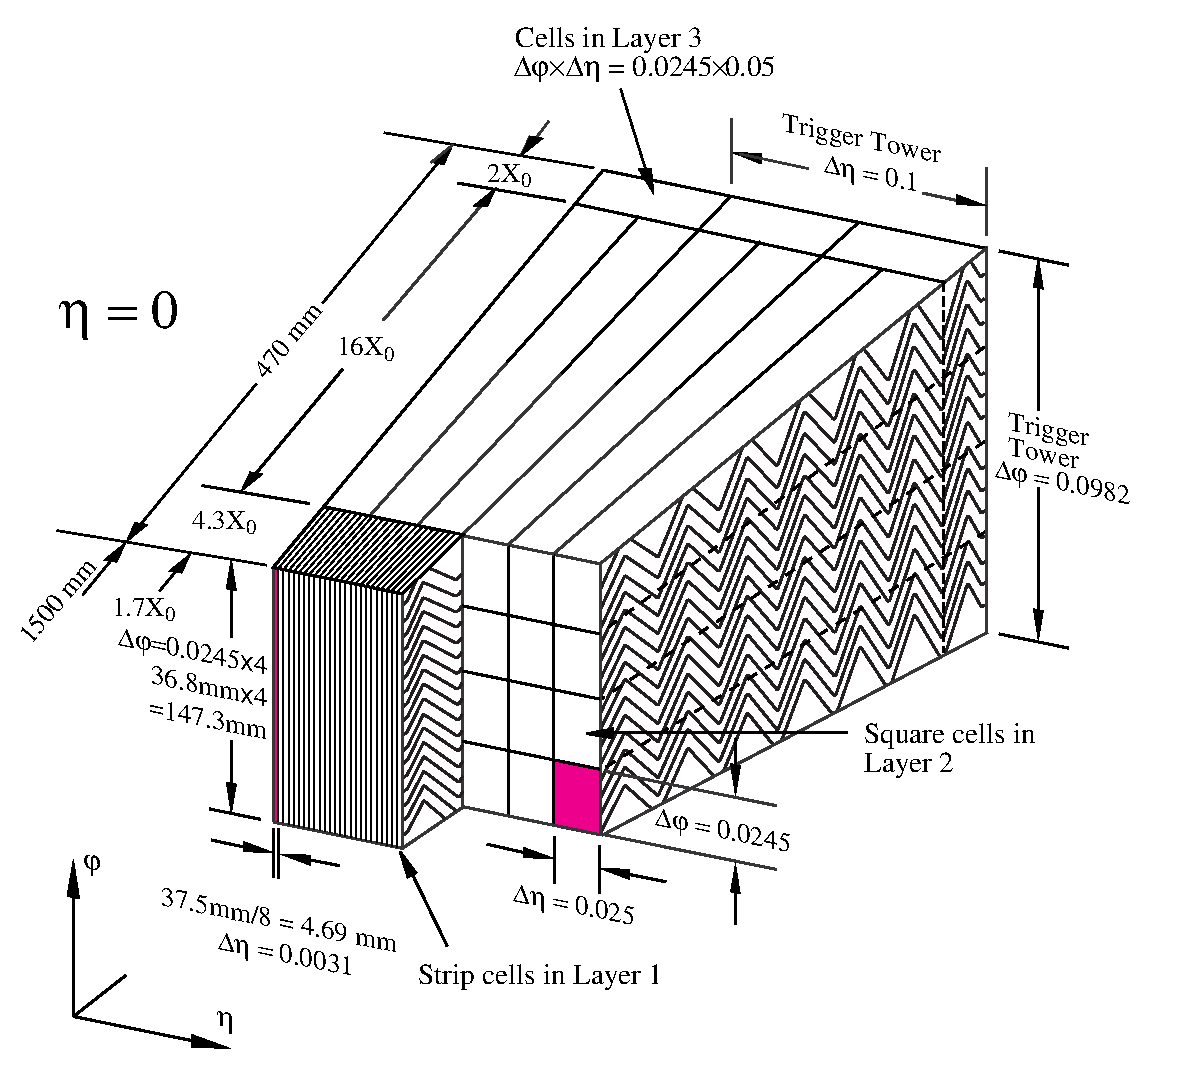
\includegraphics[width=0.48\textwidth]{detector/figures/caloLAr2}}
	\subfigure[]{\label{fig:calotile}
  	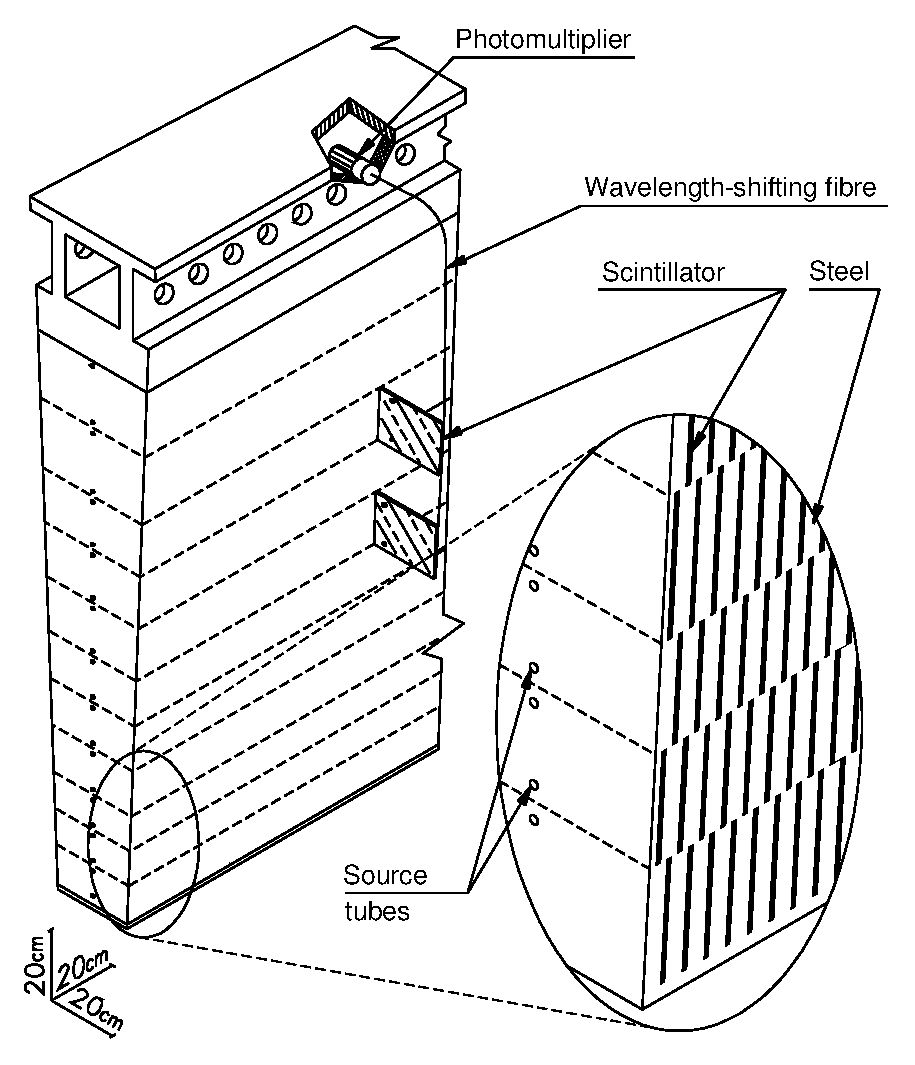
\includegraphics[width=0.38\textwidth]{detector/figures/caloTile}}
	\caption{(a) Schematic drawing of a module of the Electromagnetic barrel calorimeter. 
        (b) Schematic drawing of a module of the Hadronic barrel calorimeter.}
\end{center}\end{figure}


The absorbing material is lead shaped into an accordion geometry to achieve
full symmetry in $\phi$, as shown in the drawing of Figure~\ref{fig:calolar}.
Signal from the ionization produced in the liquid argon is collected
by an electrode in the middle of the active material region, fixed into
a honeycomb structure.

The thickness of the absorber layers depend on the pseudorapidity in
order to make particles entering the system with different incident 
angles cross the same amount of material.

\subsubsection{Hadronic calorimeters}\label{sec:hadcal}

Hadronic showers have typically a much longer shape than
electromagnetic ones, and need therefore in general more
interaction lenghts of material to be fully contained.
Hadronic calorimeters are therefore designed to completely
absorb high-energy hadrons, which will deposit only some (small) part of their energy 
in the electromagnetic calorimeter.



\subsubsection{Hadronic barrel calorimeter}\label{sec:hadcalbarrel}

The hadronic calorimeter in the barrel and extended barrel region, going up to
$|\eta|<1.7$, is made of scintillating tiles as active material with lead as absorber
and is commonly referred to with the name of TileCal. 
The light in the ultraviolet range that is generated in the tiles is collected through
wavelenght shifting optical fibre (Figure~\ref{fig:calotile}).

TileCal sits just after the electromagnetic
calorimeter and measures the energy and position of jets and isolated hadrons.
It is divided in depth in three layers with varying lenght (1.4, 4.1, 1.8 hadronic interaction
leghts $\lambda$ in the barrel and 1.5, 2.6, 3.3$\lambda$ in the extended barrel) and segmentation
($\Delta\eta\times\Delta\phi$ = 0.1$\times$0.1 in the first two layers,
$\Delta\eta\times\Delta\phi$ = 0.2$\times$0.1 in the third),
and in 64 slices in $\phi$, each of $\Delta\phi\sim0.1$.

The redout channels are grouped into cells that form a pseudo-projective geometry in $\eta$.

\subsubsection{Hadronic end-cap calorimeter}\label{sec:hadcalendcap}

The Hadronic End-Cap calorimeters (HEC) use copper as passive material and liquid
argon as active material, chosen for its radiation hardness in a region ($1.5<|\eta|<3.2$)
exposed to a significant amount of particle flux. Each HEC is composed by
two independent wheels with granularity varying with $\eta$: 
in $1.5<|\eta|<2.5$ $\Delta\eta\times\Delta\phi$ is 0.1$\times$0.1 in the first
two longitudinal layers,  0.2$\times$0.1 in the last one; in
$2.5<|\eta|<3.2$ $1.5<|\eta|<2.5$ $\Delta\eta\times\Delta\phi$ = 0.2$\times$0.2
in all the three samples.

The HECs collect the energy from particles that are not completely contained
in the EMECs and in particular are used to reconstruct jets and the missing transverse
energy.

\subsubsection{Forward calorimeter}\label{sec:calforward}

The Forward Calorimeter (FCal) cover the very forward region of pseudorapidity
$3.1<|\eta|<4.9$ making the calorimeter system achieve its good hermeticity
and minimize the energy losses.
It has an electromagnetic part that uses copper as absorber and two hadronic compartments
with tungsten as passive material. 




\subsection{Muon spectrometer}\label{sec:muonspec}

The most external detector system is the muon spectrometer, a combination
of toroidal superconducting magnets (Section~\ref{sec:magnets}) and precision
chambers providing a measurement of the momentum of muons in $|\eta|<2.7$ in addition
to the measurement from the ID. It is also equipped 
with an independent trigger system used for the first event triggering
stage (see Section~\ref{sec:lvl1}) active in the pseudorapidity region $|\eta|<2.4$. 

Four sub-detectors compose the muon system: Monitored Drift-Tube (MDT) chambers, 
Cathode Strips Chambers (CSC), Resistive Plate Chambers (RPC) and Thin Gap Chambers (TGC).
The layout changes in the barrel and end-cap regions, and is schematically shown in 
Figure~\ref{fig:muonSect}: in the  barrel region, chambers are arranged in three cylindrical layers around
the beam axis, one layer being inside the magnet; in the end-caps these three layers are placed 
perpendicular to the beam axis.

\begin{figure}[tb]\begin{center}
	\subfigure[]{\label{fig:muonSect2}
        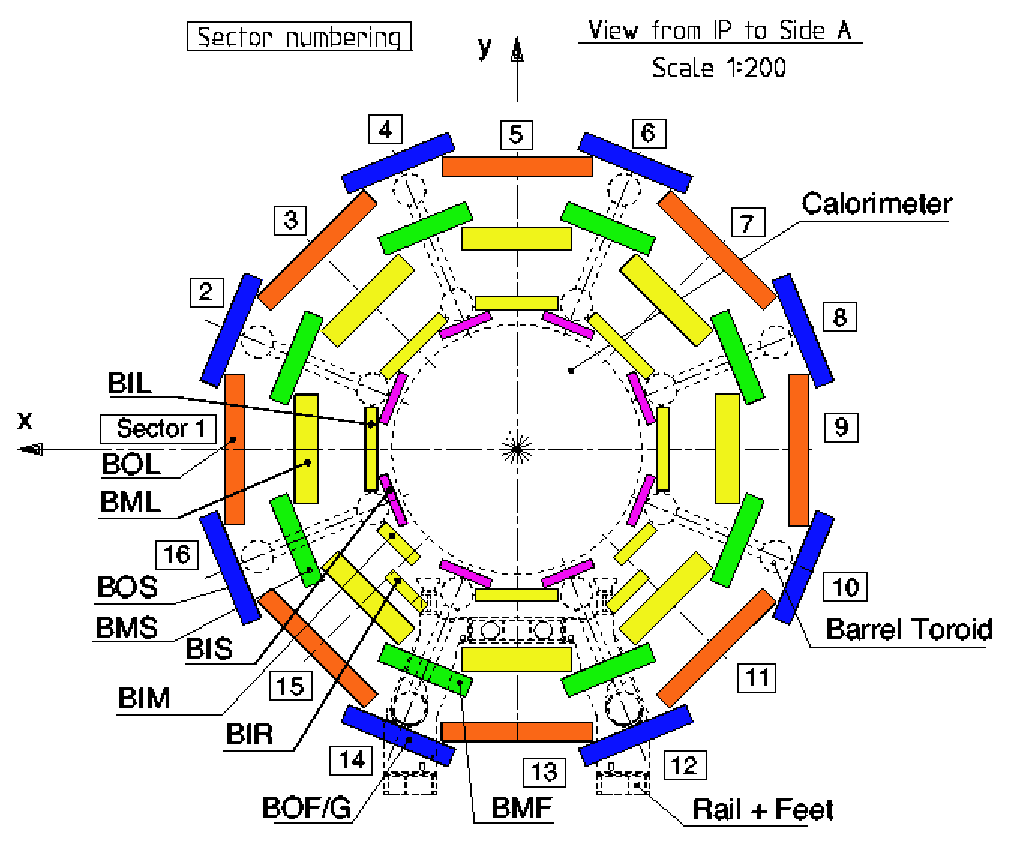
\includegraphics[width=.4\textwidth]{detector/figures/muonSect2}}
	\subfigure[]{\label{fig:muonSect}
        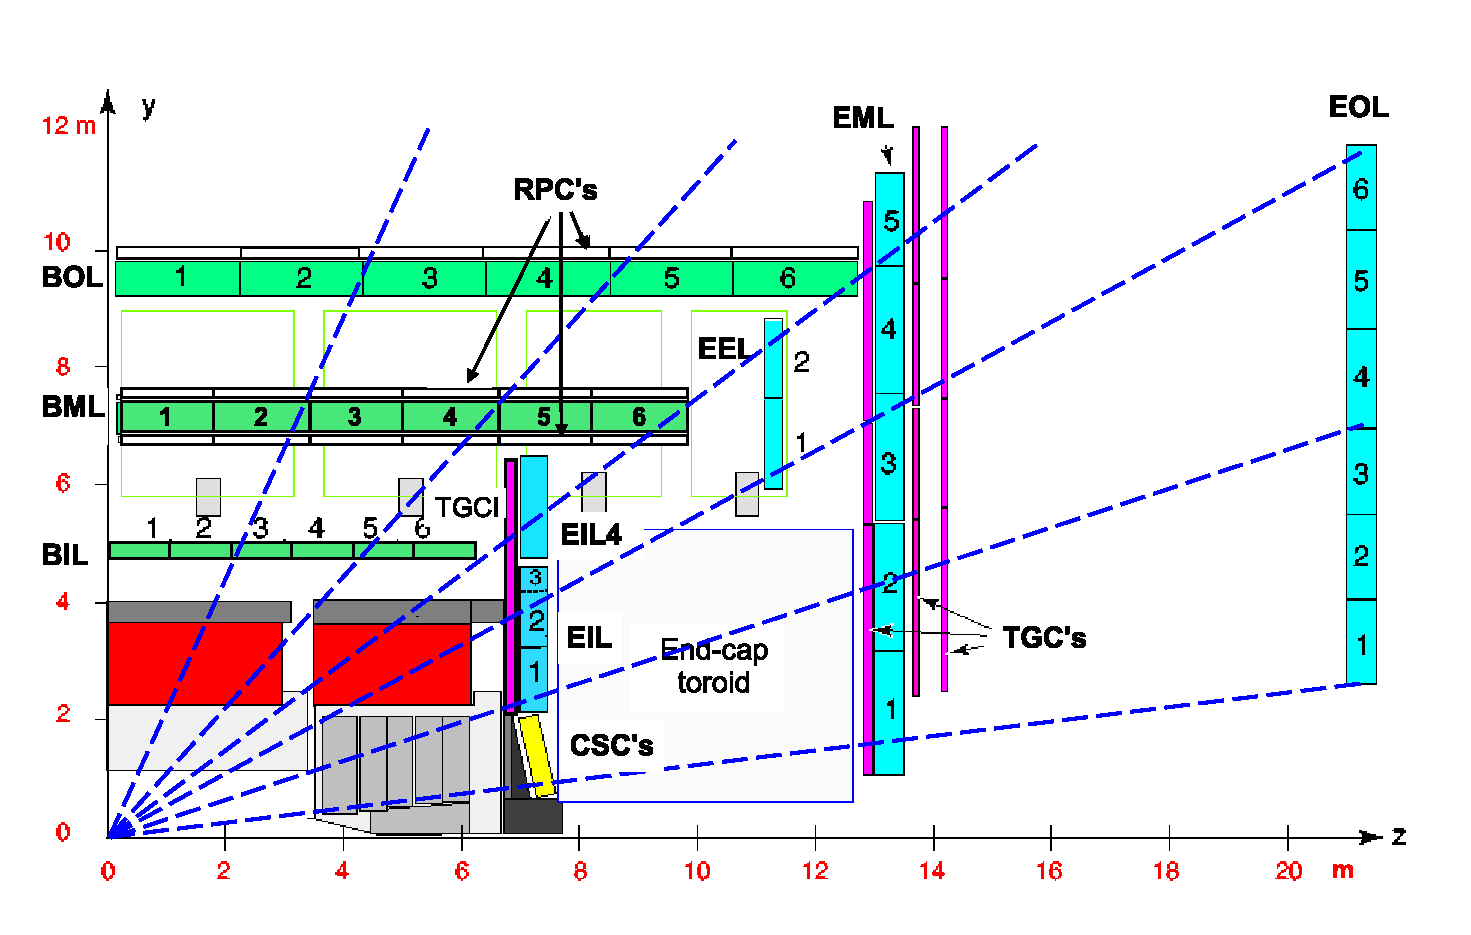
\includegraphics[width=.5\textwidth]{detector/figures/muonSect}}
	\caption{(a) Cross section of the barrel muon system. (b) Lateral section of the muon system. 
        Barrel MDTs are shown in green, end-caps MDTs in light blue, CSC in yellow, 
        TGCs in magenta, RPCs in white.%  (From \cite{Aad:JINST})
        }
\end{center}\end{figure}


\subsubsection{Detection chambers}

MDTs and CSCs are used to detect muons in the pseudorapidity regions $|\eta|<2.0$ and
$2.0<|\eta|<2.7$ respectively. MDTs are proportional chambers constituted by 
pressurised drift tubes made of aluminium with a diameter of 30~mm and lenght varying from 0.9~m to 6.2~m. 
The gas mixture in them is 93\% argon and 7\% carbon dioxyde, the anode is a 50~$\mu$m
tungsten-rhenium wire producing a radial electric field. Each chamber is composed by 
a group of six or eight tubes placed transverse to the beam axis. This number of tubes allows
for a very good track reconstruction and high reduction of the fake tracks from random 
associations of background hits, providing a resolution on position of 80 $\mu$m.
%gives a momentum  resolution $\sigma_{p_{T}}/p_{T} < 10^{-4}$~\GeV$^{-1} \cdot p_{T}$ for tracks with $p_{T} > $300~GeV.


The CSCs are used at higher $\eta$ to better cope with the higher particle flux.
They are arranged in a system of two disks with eight chambers each. Each chamber
contains four multiwire proportional chambers (the CSCs) with wires oriented in the radial direction,
spaced by 2.5~mm and in the same gas mixture of argon and carbon dioxyde as the MDTs.
The cathode strips are oriented one perpendicularly to the anode wires (and gives the precision coordinate)
and the other parallel to the wires (and gives the transverse coordinate).
The resolution provided by the interpolation between the charges induced on neighbouring cathode strips
ranges between 50 and 70 $\mu$m.

\subsubsection{Trigger chambers}

For trigger purposes detectors with faster response than drift tubes are needed\footnote{Drift-time in tubes with a diameter of 
$\mathcal{O}\sim 10$~mm can be of $\sim500$~ns, too long with respect to the 25 ns spacing of the bunch crossings.}.
MDTs and CSCs are then coupled with special layers of trigger chambers: in the barrel region, the MDT's second layer
is covered on both sides by RPCs, while MDT's third layer is covered by a RPC alternatively on the inner and outer side;
in the end–caps, TGCs cover the inner side of MDT's first and third layers. 

A RPC is a detector with a gas-gap between two resistive bakelite plates separated by 2~mm and containing
a gas mixture of C$_{2}$H$_{2}$F$_{4}$ (94.7\%), Iso-C$_{4}$H$_{10}$ (5\%) and SF$_{6}$ (0.3\%). 
RPCs measure six points per coordinate for each particle, quickly collecting the avalanches with two 
orthogonal sets of pick-up strips that provides a position resolution of 1 cm in each plane and 1 ns time resolution,
allowing for individual bunch crossing discrimination. Also RPCs provide the $\phi$ coordinate for the tracks in
the final analysis, since MDTs only give the $\eta$ coordinate.

TGCs are similar to CSCs, have 1.8~mm wire-to-wire separation and 
1.4~mm wire-to-cathode separation. They use a highly quenching gas mixture of CO$_{2}$ 55\% and n-C$_{5}$H$_{12}$ 45\%
and provide  a spatial resolution of about 1~mm and a time resolution of 5~ns.

\section{Forward sub-detectors}\label{sec:forward}

ATLAS is equipped with some detectors in the forward regions to perform additional measurements or
monitoring studies. In particular, the Minimum Bias Trigger Scintillators (MBTS), that are somehow
embedded in the structure of TileCal extended barrel modules (see Figure~\ref{fig:extendedbarrel})
and share with it the readout electronics, as they are also read by wavelenght-shifting fibers.
The MBTS consist of 32 scintillator paddles assembled in two disks covering the pseudorapidity region
$2.09<|\eta|<3.84$ and are used for trigger purposes to detect minimum bias activity during the first
runs of the LHC. 

MBTS are also used for relative luminosity measurements, but there are two detectors specifically
built to determine the luminosity delivered to ATLAS: LUCID and ALFA. LUCID (LUminosity measurements
using Cerenkov Integrating Detector) is made of 32 tubes surrounding the beam pipe 17~m
far from the interaction point on both sides of ATLAS and measures the luminosity bunch by bunch.
ALFA (Absolute Luminosity For ATLAS) is only activated during special runs, and consists of 8 
scintillating fibers detectors placed at 240~m from the interaction point inside roman pots, above and
below the beam pipe.

Another luminosity monitorer is the Zero-Degree Calorimeter, whose main purpose is to determine the centrality of heavy-ion
collisions. Placed at 140~m from the interaction point on both sides of the beam axis, is made of quartz rods
alternated with tungsten plates.

Finally, the Beam Condition Monitor (BCM) is made of two sets of diamond sensors located 184~cm close
to the interaction point along the beam and 5.5~cm close along $R$. Its task is to detect beam losses,
potentially harmful for ATLAS, and in that case to alert LHC in order to stop the accelerator.



\begin{figure}[tb]\begin{center}
	\subfigure{
  	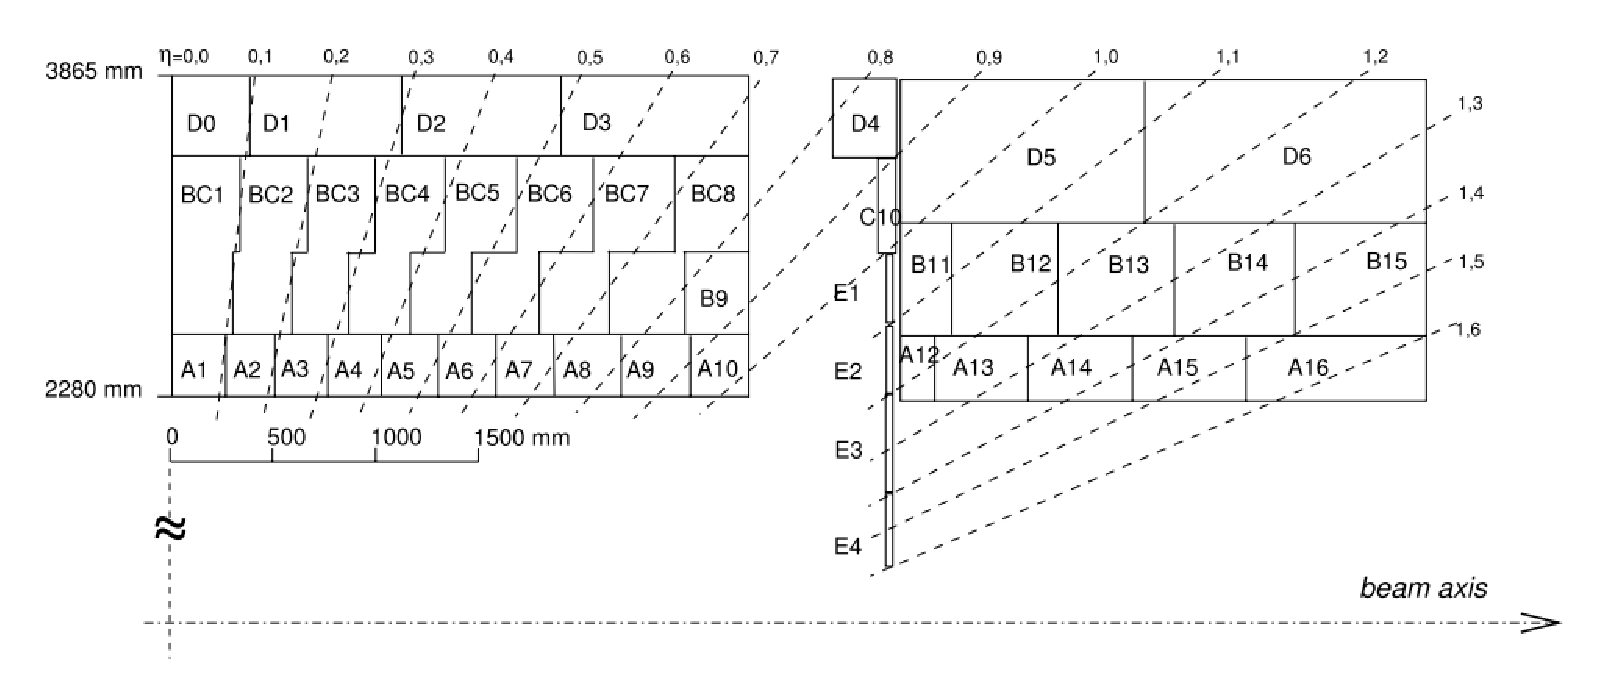
\includegraphics[width=0.\textwidth]{detector/figures/extendedbarrel}}
	\caption{Schematic of a section of TileCal barrel and extended barrel modules, with the
        cells division. The parts labelled with ``E'' are the MBTS.\label{fig:extendedbarrel}}
\end{center}\end{figure}


\section{Trigger system}\label{sec:trigger}

It was already introduced at the beginning of this Chapter the issue
faced by LHC experiments of dealing with a huge amounts of events
at very high frequencies. We remind that considering the nominal LHC
luminosity of \highL\ a rate of interactions of 40~MHz is expected!
This poses serious technical difficulties as the maximum frequency
at which data can be recorded is limited to 200~Hz considering the
limited capacity for storage.

ATLAS developed a trigger system able to reduce by a factor of 10$^6$
the amount of data to be kept by selecting only interesting physics events.
The system is divided in three levels characterized by increasing sofistication
and diminishing speed. At the very first indeed we will need a really quick and
simple criterium to reject uninteresting events. The reduced information can then be
processed with somehow slower logic by the other two High Level Triggers (HLT).
A drawing of the system is shown in Figure~\ref{fig:trigger}.

\begin{figure}[tb]\begin{center}
	\subfigure{
  	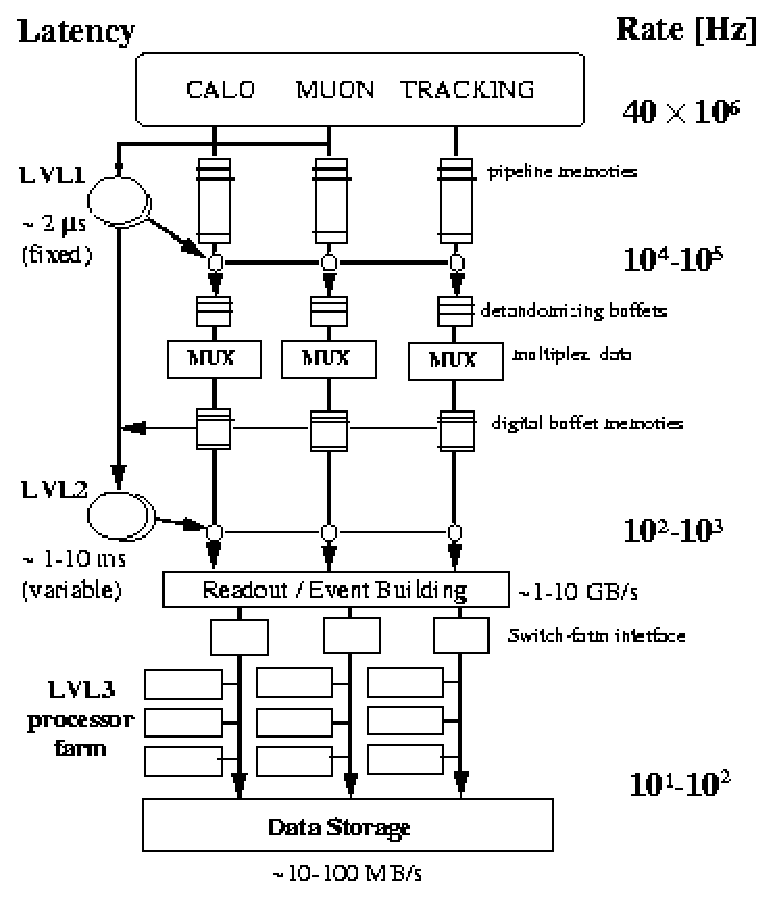
\includegraphics[width=0.5\textwidth]{detector/figures/triggerscheme}}
	\caption{Schematic drawing of the three-level trigger system of ATLAS.\label{fig:trigger}}
\end{center}\end{figure}

Most of the trigger chains used for physics are un-scaled in the
sense that all the events passing the selection are kept, but there
are also pre-scaled trigger chains that contain either too many events
or events considered not physically interesting. These trigger chains
are used for checks or calibration rather than physics analysis, and the
prescaling value $P$ means that of all the events that would have passed 
the trigger, $1/P$ were accepted.

With the term ``trigger chain'' we refer to the sequence of selections
defining a certain trigger object, with a naming convention like:
\begin{equation*}\label{eq:}
{\rm [LEVEL][N][TYPE(S)][THRESHOLD][ISOLATION][QUALITY]},
\end{equation*}
where the components, from left to right, are: the trigger level used; the
multiplicity of the type; the object candidate; the threshold applied to
the transverse momentum or energy of the object candidate; the object isolation;
the severity of the final algorithm requirements (this applies only to the Event
Filter level).

Trigger chains define a {\it trigger menu}, where they are associated to their
prescale value $P$, and which is chosen based on the physics program of the
data taking period taking into account the LHC luminosity. 

Defining the data taking period time unit as ``Luminosity Block'' (LB), typically
a few minutes of  data taking, information on beam conditions, detector performance 
and events passing any of the trigger chains of the trigger menu are stored
to be then used in the analyses. All the LB occurring between the start and the
end of a stable beam collision period compose a ``run''. Runs are finally grouped
in ``Data Periods'', labelled with capital letters (``Period A'', ``Period B'', {\it etc}.),
when they pertain to the same general detector condition, machine configuration and
trigger menu.




\subsection{Level 1 trigger}\label{sec:lvl1}

The Level 1 trigger (L1) is completely based on the hardware of the detector,
taking information from calorimeters, from the muon spectrometer trigger
systems RPC and TGC (Section~\ref{sec:muonspec}) and from the MBTS (Section~\ref{sec:forward}) 
at 40~MHz (the frequency of the beam crossing) and reducing it to 75~kHz by choosing events with high
transverse momentum or high missing transverse energy.

Using dedicated fast front-end electronics (the typical decision time being less than
2~$\mu$s), calorimeter cells are analogically 
summed to build calorimetric towers which, if having an energy higher than a 
certain threshold, will activate a trigger chain.

These trigger chains will then be combined with the information from the
muon spectrometer to form the so-called Region of Interest (RoI) that is
passed to the next trigger level.


\subsection{Level 2 trigger}\label{sec:lvl2}

Starting from the RoI, the Level 2 trigger (L2) will reduce the 75~kHz to
3.5~kHz of events with an average decision time of 40~ms. At this
stage the information from the trackers is incorporated to the RoI
to build candidate object (electrons, photons, muons) and 
better obtain its position and energy with simplified algorithms
quick enough to respect the limit on the decision time.

\subsection{Event filter}\label{sec:lvl3}

The last trigger, Level 3, is called Event Filter (EF) since
at this point the physics objects are built using the same
algorithms as the off-line reconstruction, with looser selections. With an execution time
amounting to 4~s, the EF reduces the event rate to the goal value
of 200~Hz.
Events passing the EF are assigned to {\it streams} defined to separate
the events into different datasets for different analysis interests, e.g.
electron streams, muon streams, jet streams {\it etc}.

As an example, one of the trigger chains used in our analysis is 
\texttt{EF\_mu24i\_tight}: it selects events at the EF level with one 
muon with $p_T>24$~\gev\ and some isolation requirement which passes
the muon reconstruction algorithm cuts defined as ``tight''
(more on event reconstruction is reported in the dedicated Chapter~\ref{chap:objects}).

\section{Data Quality}\label{sec:daq}

The totality of p-p collisions recorded by ATLAS, which differs from the amount
delivered by the LHC because of data-taking inefficiencies, is still
not 100\% usable by physics analyses. Indeed, every subdetector needs to
perform some routine checks %(usually done by PhD students) 
on the quality of the data they recorded in order to certify that its performace
was conform to the expectations. So-called ``Good Runs Lists'' (GRL) are
compiled stating for each LB what was ``OK'' and what not.
The single analyses will then decide which GRL to use, based on their specific
needs of the individual subsystems.
